\documentclass[]{report}
\usepackage{geometry}
\usepackage{graphicx}
\usepackage{xcolor}
\geometry{a4paper, top=2cm, bottom=2cm, left=2.5cm, right=2.5cm,  heightrounded, bindingoffset=5mm}
\usepackage[T1]{fontenc}
\usepackage[utf8]{inputenc}
\usepackage{titlesec}
\usepackage{subfig}
\usepackage{amsmath}
\usepackage{wrapfig}
\title{\huge \textbf{Frequent Itemsets Mining} 
	\\ \LARGE \textit{SON Algorithms: a MapReduce Approach}}
\author{\textit{Francesco Martini}}
\date{\textit{A.A. 2020/2021}}
\captionsetup[subfloat]{labelformat=empty}

\begin{document}
\maketitle
\chapter*{\huge Preface}

	This report has the aim to describe the theoretical context and the technical aspects behind the development of this project whose overall goal was the implementation of the SON algorithm for frequent itemsets mining. \\
	The algorithm has been parallelized exploiting the MapReduce model and its performance has been compared with the one of Apriori which represent the most common and simple non-parallelized approach used to solve the task mentioned before. \\
	To ensure a fair comparison, an open source library has been used to provide an efficient implementation of Apriori.
	This library and its documentation can be found at the following link:
	
	\begin{itemize}
		\item https://www.philippe-fournier-viger.com/spmf/
	\end{itemize}     

\chapter*{\huge Theoretical Premises}

	The two algorithms described in this report have a common goal: the extraction of frequent itemsest from a transactional dataset.
	The theoretical concepts which surround this task (and the way each algorithm achieves it) will be briefly covered in the following sections in order to dedicate the next chapters to the more technical aspects of the project.     

\section*{Transactional Model and Freqent Itemsets:}
	
	With \textbf{Transactional Model} we mean a particular kind of dataset which contains, as the name suggest, transactions. In particular, a \textbf{transaction} is a collection of elements, commonly named \textbf{item}, which are selected from a global set \textbf{\textit{I}} of all the items (ex. the set of products in a supermarket). Given a transactional datset \textit{TD} we can imagine \textbf{\textit{I}} to be the set of all items which occur at least in one transaction of \textit{TD}.
	\\ It is also possible to increase the complexity of the transactional model by introducing concept like items order or timestamps which lead us to the definition, for example, of 'temporal transaction'. For the purpose of the project these cases will not be considered and, in particular, we will define a transactions \textit{t} as any subset of \textbf{\textit{I}} implying that the items contained in \textit{t} will appear without repetition and without an order. Consequently the only operation we can do with two items \textit{i\textsubscript{1}} and \textit{i\textsubscript{2}} is to check if they are the same item. That being said, a transactional dataset could be also represented as a many-to-many relation between a set \textit{T} of transaction identifiers and the previously defined set \textbf{\textit{I}}.  \\ 
	Similarly to a transaction, an \textbf{itemset} is defined, in this scenario, as a subset of \textbf{\textit{I}}. The difference here is that, for an itemset \textit{itms}, it is possible to compute its \textit{Support} wrt a transactional dataset \textit{TD} through the following equation:
	\vspace{0mm}\\
	\begin{equation}
	Support(itms, DT) = \frac{Count(itms)}{|DT|} 
	\end{equation}    
	...where \textit{|DT|} represent the number of transactions in the transactional dataset and \textit{Count(itms)} represent the number of transactions in which, the itemset \textit{itms}, appears as subset. It's also possible to choose a threshold value \textit{ps} which can be used to decide if an itemset \textit{itms}\textsubscript{1} is a \textbf{frequent itemset} or not according to the following definition:
	\vspace{0mm}\\
	\begin{equation}
		IsFrequent(itms\textsubscript{1}, DT)=\begin{cases}
			Yes & \text{if $Support(itms\textsubscript{1}, DT) \geq\, $\textit{ps}}.\\
			No & \text{otherwise}.
		\end{cases}
	\end{equation} 
	Frequent itemsets are particularly interesting for what they represent and for their \textit{monotonicity} property. In fact, they highlight the sets of items which usually occur together in the dataset's transactions. This concept find many application even in real life where, as instance, the transactional dataset could be the collection of purchases made by the clients of an online-store and the set \textbf{\textit{I}} could be the set of all store's articles. In this scenario the frequent itemsets would correspond to the articles the clients usually buy together: a concept of obvious interest for every store-owner. Therefore, what's left to do, is to find a way to compute these particular itemsets. The first basic approach is to try an exhaustive-research computing all the possible itemsets and checking for all of them if they are frequent or not. This approach, as simple as it sounds, can't be practically applied: the number of possible itemsets, related to a set \textbf{\textit{I}} of \textit{k} items, is equal to the number of all possible combinations of \textit{n} elements of \textbf{\textit{I}} with the integer \textit{n} in the range [1..k]. If we consider that usually the cardinality
	of set \textbf{\textit{I}} exceeds the hundred of elements, this number of itemsets (which also correspond to the number of all possible subset of \textbf{\textit{I}}) becomes clearly too big to be processed. Luckily, it's possible to reduce drastically the complexity of this computation wrt the average-case exploiting the \textit{monotonicity} property.
	\\
	\hspace{-5mm}
	\begin{tabular}{ | l | }
		\hline \vspace{-3mm}\\
		\textbf{\textit{Monotonicity Property:}}\\
		\hline \vspace{-3mm}\\
		If a given itemset \textit{itms\textsubscript{1}} is said to be frequent, then all its subsets are also frequent itemsets.\\
		At the same time, if an itemset \textit{itms\textsubscript{2}} is not frequent, than all its supersets will not be frequent \\as well. \\
		\hline	    
	\end{tabular}            
	\\ \vspace{3mm}
	\\
	Furthermore, a frequent itemset whose supersets are all not frequent is called \textbf{maximal}. The collection of all maximal frequent itemsets for a dataset \textit{DT} and a support threshold \textit{sp} is sufficient to describe all frequent itemset of the dataset: the ones that are not explicitly listed correspond to all the subsets of these maximal frequent itemsets. 
	This property represent the foundations on top of which is built the Apriori algorithm described below. 

\section*{Apriori Algorithm:}

	The main idea behind the \textbf{Apriori} algorithm is to exploit the monotonicity property to reduce the number of itemsets to check. \\ As first step, the algorithm check right away if there are frequent itemsets which contain only one element. It's reasonable to suppose that some particularly rare items will not appear in the dataset with the sufficient support needed to surpass the problem threshold thus, their corresponding itemsets, will not appear as 'frequent'. The consequences of this are that it is possible to skip the checking phase for all the supersets which contain a non-frequent item. In particular this principle is also valid for the itemsets of two elements: it's, in fact, possible to compute the candidate couples starting from the single frequent items. Only after this preliminary computation, a filtering step could be applied in order to keep, again, only the frequent sets. \\
	This pattern could always be applied for itemsets of size \textit{k}+1 in order to discover which of them are frequent given the collection of frequent itemsets of size \textit{k}. The Apriori algorithm, simply keeps repeating these steps until the collection of candidate itemsets becomes empty. \\
	It's worth noting that this technique, in the worst case scenario, will perform an exhaustive-research for all possible itemsets. In fact, the improvement given by this approach are deeply linked with the main parameter of the problem: the support threshold \textit{sp}. Luckily the worst-case scenario will happen only if one of these two cases is verified:
	\begin{itemize}
		\item \textit{sp} is 0;
		\item at least one transaction contains all the possible items in \textbf{\textit{I}} AND \textit{sp} is sufficiently small. 
	\end{itemize}     
	This two cases are both not much interesting because the first represents a degenerate case which will always result in the same answer to the original problem ('all possible itemsets are frequent'); the second, instead, requires a dataset structure which isn't common in real applications where usually the transactions maximal size is way smaller then the cardinality of \textbf{\textit{I}}.     
	The performance of the algorithm also depend on: the usage of memory, the implementation of the 'joining step' where the candidate itemsets are chosen, the structures used to store data. These aspects are beyond the scope of this chapter and, for this reason, they won't be covered.
	
\section*{SON Algorithm:}   		

	The SON (Savasere, Omiecinski,
	Navathe) algorithm represent an alternative approach to compute the frequent itemsets of a transactional dataset. This algorithm doesn't provide a computational method to resolve this problem but simply suggest to split the original dataset in many chunks in order to generate many smaller problems of the same nature of the original one. In order to do so is also necessary to rescale the problem threshold \textit{sp} into a new value \textit{p}\textsubscript{i} proportional to the dataset's sample \textit{DS}\textsubscript{i} and its \textit{k}\textsubscript{i} value which represents the portion of transactions in \textit{DS}\textsubscript{i} wrt the whole dataset:
	\begin{equation}
		p\textsubscript{i} = k\textsubscript{i}sp
	\end{equation}
	 \\
	After splitting the dataset the algorithm will solve each single sub-problem in order to generate multiple collections of frequent itemsets computed for each sample \textit{DS}\textsubscript{i} wrt the proper threshold \textit{p}\textsubscript{i}. To accomplish this goal we can use any algorithm for frequent itemsets extraction (like Apriori). At this point it's possible to merge the collections of frequent itemsets found and search for the ones that are really frequent wrt the whole dataset.\\
	The strength of SON algorithm lies in the fact that, if we split a dataset in many small chunks, it become possible to store all the transactions of the given chunk in the main memory. Thanks to this we could apply an itemsets mining algorithm without the overhead which comes with the usage of the disk. SON also ensures that the solution we found is correct and complete thanks to the following property:      
	\\
	\\
	\begin{tabular}{ | l | }
		\hline \vspace{-3mm}\\
		\textbf{\textit{Chunks Property:}}\\
		\hline \vspace{-3mm}\\
		Given an itemset \textit{itms} which is \textbf{frequent} wrt a dataset \textit{DT} and a support threshold \textit{sp}, if \textit{DT} is\\ 
		splitted in \textit{n} subset such that at each subset \textit{DS}\textsubscript{i} correspond a threshold \textit{p}\textsubscript{i} computed as in (3)\\ and is true that:\\
		- $\forall$x,y  with x$\ne$y: \textit{DS}\textsubscript{x}$\cap$\textit{DS}\textsubscript{y} = $\emptyset$\\
		- \textit{DS}\textsubscript{1}$\cup$\textit{DS}\textsubscript{2}$\cup$...$\cup$\textit{DS}\textsubscript{n} = \textit{DT}
			\\ then \textit{itms} must be frequent wrt at least one subset \textit{DS}\textsubscript{k} and its threshold \textit{p}\textsubscript{k}.\\ 
		\hline	    
	\end{tabular}            
	\\ \vspace{3mm}
	\\
	It's important to underline that, when performing set operations between chunks, we are considering transactions composed by a set of items AND an unique identifier, thus, if \textit{DT} contains two transactions with same items, they will still differ by their identifiers.
	That being said, the support of an itemset wrt \textit{DT} can be written as the average of its supports computed for all the chunks and weighed by the related \textit{k} values: if the support average is above \textit{sp} then SON algorithm will find this itemset as frequent wrt at least on chunk and it will be reported in the final collection of candidate itemsets ensuring, as stated before, its presence in the solution.
	 
\section*{MapReduce Approach:}
	
	SON algorithm, thanks to its structure, can be easily adapted to a MapReduce environment. To do so is necessary to split the computation in 2 cycles of MapReduce as follow:
	\begin{enumerate}
		\item \textbf{First \textit{Map} Step:} the dataset file is divided in chunks and each one of them is passed to the first Mapper whose role is to apply the mining algorithm on the fraction of dataset recived as input having care of lowering the support threshold according to the size of the file's sample received. The output would be a set of key-value pairs (\textit{F},1) where \textit{F} is a frequent itemset wrt the sample (the value is irrelevant).
		\item \textbf{First \textit{Reduce} Step:} each task will receive a set of itemsets as keys and it does nothing more than returning that keys as output values: these are the candidate itemsets appeared at least one time in the samples.   
		\item \textbf{Second \textit{Map} Step:} this step takes as input a fraction of the original data file along with all the candidate itemsets computed in the last Reduce phase. The goal, here, is to count the occurrences of each candidate itemsets in the given sample's transactions. The output would be a collection of (\textit{C}, \textit{v}) pairs where \textit{C} is a candidate itemset and \textit{v} is the number of occurrences computed wrt the dataset's sample received as input by the function.
		\item \textbf{Second \textit{Reduce} Step:} 
		with this last Reduce step, the algorithm could sum, for each candidate itemset, the associated values and choose to keep only the ones with sum greater or equal then \textit{sp} (the support threshold of the problem). The output pairs will be represented by the the couples (\textit{CF}, \textit{s}) where CF is the frequent itemset and \textit{s} is its occurrences count wrt the whole dataset. 
	\end{enumerate}	
	In order to keep everything simple the algorithm will consider the occurrences count of the candidate itemsets instead of their support: these two values are in fact strongly correlated and they can be considered equivalent wrt their roles in this problem (it's possible to ignore the support normalization factor represented by the size of the dataset).	 	
	
\chapter*{\huge Environment and Datset}

	The project's code has been developed and tested in a Windows (10 Pro) machine with 8GB of RAM and a Ryzen 5 CPU model. The code is meant to run in an HDFS cluster thus it has been necessary, in order to simulate this kind of environment on a single machine, to rely on the frameworks described below.   

\section*{Hadoop:}

	Docker virtualization framework has been used to simulate the environment of a cluster. Docker engine has been update to the 19.03.13 version and it has been installed along with WSL 2 to allow communications between the windows-based client and the linux-based server responsible for containers management. Cloudera image has also been downloaded to generate the proper container necessary to simulate a single-node HDFS environment. This image has been pulled from Docker Hub in order to have access to the included CDH (Cloudera distribution of Apache Hadoop) whose hadoop version is the 2.6.0-cdh5.7.0.

\section*{Datasets:}

	All the datasets used for the project have been generated by the IBM's open-source tool available at the following link:
	\begin{itemize}
		\item https://sourceforge.net/projects/ibmquestdatagen/
	\end{itemize}
	This tool is no longer supported and it was originally designed to generate transactional datasets in many formats. It comes as a zip file containing several cpp functions and a .sln (Solution file) that can be open as a VisualStudio project to generate the datasets. As suggest in the README file, it's necessary to set up the project debug parameters in order to generate a new dataset. These parameters shall be added under "Debug $\rightarrow$ $<$nameproject$>$ Properties... $\rightarrow$ Configuration Properties $\rightarrow$ Debugging $\rightarrow$ Command Arguments" and shall follow the format below:
	\begin{itemize}
		\item \textbf{lit -ascii -ntrans XX -tlen YY -nitems ZZ > TXXLYYNZZ.txt}
	\end{itemize}
	Where:
	\begin{itemize}	
		\item \textbf{lit:} key value used to indicate the desired kind of dataset (in this case a standard transactional dataset);
		\item \textbf{-ascii:} encoding used to write the dataset;
		\item \textbf{-ntrans:} number of transactions (XX x 1000 transactions will be produced);
		\item \textbf{-tlen:} average number of items per transaction (YY); 
		\item \textbf{-nitems:} size of set \textbf{\textit{I}} of all items (it will contain ZZ x 1000 different elements);
		\item \textbf{> TXXLYYNZZ.txt:} output file where data will be written.
	\end{itemize}
	Some additional files will be generated by the script. These can be ignored. The final result is a dataset with the format shown in the image below where, as instance, \textbf{-ntrans} parameter is set to \textbf{n}. 
	In particular we will see, for each line, two numbers: the first is the transaction identifier, the second represents one of the items contained in that specific transaction. The image shows the first and the last part of the datasets which of course, in a real scenario, will contain a proper identification number instead of \textbf{n} or \textbf{n-x}. 
	\\\\\\
	\begin{figure}[h]
		\centering
		\hspace{1cm}
		\subfloat[]{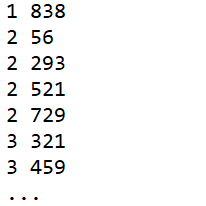
\includegraphics[scale=1]{./img/dt1}}
		\hspace{1mm}
		\subfloat[]{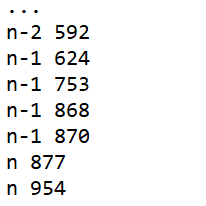
\includegraphics[scale=1]{./img/dt2}}
		\hspace{1mm} 
	\end{figure}
	\vspace{-1.0cm}\\
	In general, IBM's tools, does not generate the exact number of instances specified by the parameters but a slightly lower number. The reasons behind this behavior has not been investigated because not really interesting wrt the goal of this project. It's important to notice that datasets generated in this way will never have duplicate items within the same transaction. \\   
	Several input-files have been generated thanks to this tool, each one with different parameters configuration. In particular, in the proper project directory "datasets", is possible to find:
	\begin{itemize}	 
		\item \textit{T100L10N3.txt:} with 98355 transactions with an average length of 10 items choose within a pool of 3000 item, this represents the most used dataset during both test and performance-measurement phases;
		\item \textit{T300L30N0.1.txt (\textbf{archive}):} this dataset has been used only in the performance-measurement phase; it includes 300000 transactions with an average length of 30 items (values range [0-99]) for a total volume of 87MB (24MB after filtering step); 
		\item \textit{T1000L20N3.txt (\textbf{archive}):} contains almost 1 million transactions with an average length of 20 items, the weight of the resulting filtered dataset is about 89MB.
	\end{itemize}
	Smaller datasets have been generated for debugging purpose: these will be included in "datasets" directory but not discussed in this report. 
	Instead, it's worth underling that the format of the datasets listed above it's not the one expected by the Apriori algorithm implemented by spmf.jar.
	In order to use this library, an input dataset must list the content of a transaction (the items) all in one line such that each line of the file will correspond to a different transaction: the identifier now will be implicitly represented by the number of the current line. If we apply this format to the dataset in the figure above we obtain the following: \vspace{-0.4cm}\\
	\begin{figure}[h]
		\centering
		\subfloat[]{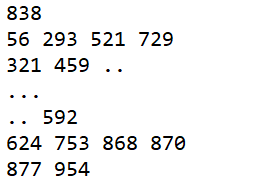
\includegraphics[scale=1]{./img/dt3}}
	\end{figure}
	\vspace{-0.5cm}\\
	To ensure a correct parsing it's also necessary to remove everything except for digits, space and the end-line character (this include the removal of tab character). For this reason "datasets" directory contains also:    
	\begin{itemize}	 
		\item \textit{test\_small.txt:} originally named 'contextPasquier99.txt', is the dataset used as example in the documentation page of the spmf library;
		\item \textit{test\_big.txt:} this dataset is the filtered version of \textit{T100L10N3.txt}; 
		\item \textit{test\_verybig.txt (\textbf{archive}):} is the filtered version of \textit{T1000L20N3.txt}.
	\end{itemize}
	From now on we will consider the first kind of datasets as input for the MapReduce job and the second as input for Apriori.

\chapter*{\huge Project Structure And Code}   		

	\begin{wrapfigure}{r}
		{6cm}
		\vspace{-0.3cm} 
		\hspace{1mm}
		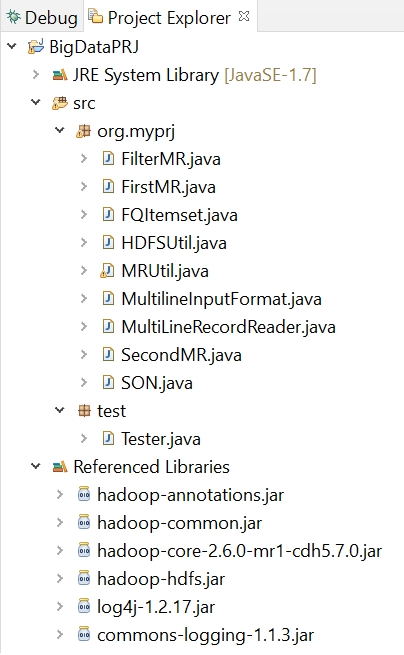
\includegraphics[width=6.5cm, height=12cm]{./img/pe}
	\end{wrapfigure}

	As suggested by the image, the project has been entirely developed in java with the support of Eclipse IDE. In order to compile the code and make the resulting .jar effectively executable in hadoop environment, it has been necessary to set java JRE to the 1.7 version and to import some external libraries listed under "Referenced Libraries" in the image and stored in the project directory "lib" (along with spmf.jar).\\
	Java test file has been separated by the other scripts that are specific for the MapReduce job. This last group of files are all in the same package and their content has been organized based on the role that the inner classes and methods cover in the project. \\
	Following this principle, \textit{SON.java} contains the main method and the driver class whose role is to manage the entire job flows. Then \textit{FirstMR.java}, \textit{SecondMR.java} and \textit{FilterMR.java} will contain the implementation of the different mapper and reducer classes. Each one of these file contains both mapper and reducer specific for the given computational step of the algorithm: this choice has been made mainly to have both map end reduce methods under control while adding a new feature or debugging. To keep all these file as lean as possible \textit{MRUtil.java} and \textit{HDFSUtil.java} has been added: these classes contains, respectively, some methods needed to configure the MR job (and to manage the algorithm parameters) and some methods necessary to manage HDFS (whose function will be later described). The remaining files are \textit{FQItemset.java}, which implements the methods necessary to find frequent itemsets from a given set of transactions, and \textit{MultilineInputFormat.java} which has been used, along with \textit{MultilineRecordReader.java}, to split and read the input files chunk by chunk.     	 
	
\section*{SON Workflow:}

	As mentioned before, SON algorithm is intended to extract frequent itemsets from a dataset in two main computational step both of which can be executed in a parallel environment. In particular, for the first step, the algorithm need to know the total number of transactions in the input file. In order to compute this number, an other preliminary map-reduce cycle has been added to the algorithm workflow.
	This initial phase has the goal to filter the dataset changing is format and counting all its transactions. The final format will be equal to the one expected by spmf.jar Apriori except for the tab character that is automatically added between key and value when these are written in the output file by the framework. The datasets generated in this way represent the input needed by the filtering function of \textit{Test.java} script which will simply remove the tab characters to produce a final dataset in the format required by Apriori.
	At this point, the proper itemsets extraction phase can start: the driver class initialize a new configuration for the next jobs adding a new field where will be stored the value of \textit{\textbf{REDUCE\_OUTPUT\_RECORD}} counter. This value is taken from the previous job's counters and represents the number of transactions in the dataset. 
	The map functions of the first extraction-job will ignore the keys of the <key, value> pairs they receive as input. All the interesting information is stored, in fact, in the pairs value which contains an entire chunk of the input dataset. The chunk dimension (in number of transactions per chunk) is set either by the algorithm or by the user. Each map function has the goal to compute a list of candidate frequent itemsets: in order to do so an instance of FQItemset is generated and the extraction algorithm is applied on the chunk. The algorithm requires a threshold expressed in number of transactions: this value is computed by the map function who generates it adapting the global support threshold to the number of transactions received as input. This is possible because each map function knows the global transactions number whose value is stored in the configuration field cited above. The map function will emit as key each one of the frequent itemsets returned by the FQItemset extractor-function. These will be passed to the reduce function which will simply ignore the collection of value and re-emit the input-key as output-key along with an empty output-value.
	As soon as the candidates list is completely written on HDFS, the last MapReduce cycle can begin. The input file for this job is the same of the previous one (filtered dataset) and even the <key, value> pairs are read in the same way as before. The map function of this job has the goal to compute the occurrences of all the candidate itemsets wrt the chunk received as input value. Each mapper exploits the functions of the HDFSUtil class in order to read all the candidates from the file produced as output by the previous job. The counting is computed thanks to an utility-function in the class FQItemset and the results are emitted by the map function as pairs composed by each candidate as key and their respective count as value.  The final reduce function is very simple: it computes the sum of all the counts related to a given key (candidate itemset) and emits a pair only if the sum is greater then the problem threshold. This pair will have as key the candidate itemset (frequent itemset from now on) and as value its support in terms of occurrences and as fraction of the dataset. \\
	The following image provides an high-level description of the algorithm workflow in all its phases.
	\begin{figure}[h]
		\subfloat[]{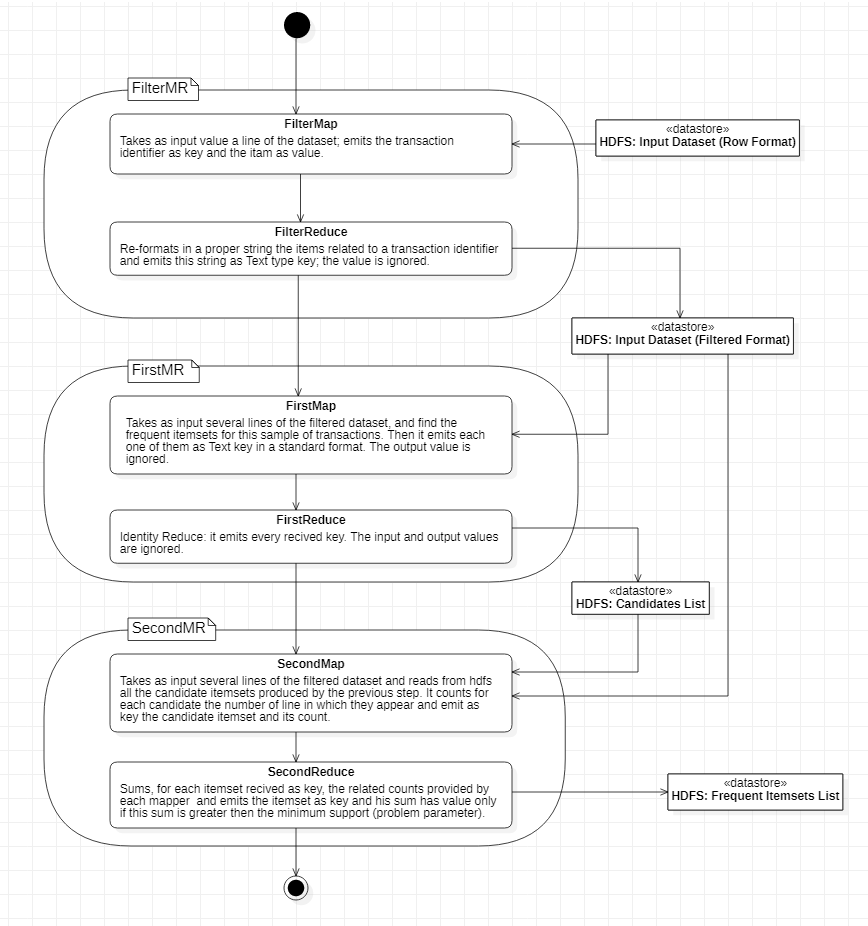
\includegraphics[scale=0.94]{./img/wf}}
	\end{figure}

\section*{SON Parameters:}
	
	The SON algorithm implemented is highly parameterized due to the fact that, other than the basic parameters proper of the frequent itemsets extraction problem, one should be able to customize the configuration of the three main MapReduce jobs.\\
	In order to run the executable son.jar from the shell of a client (connected to a cluster HDFS) is necessary to submit the following command:
	\begin{itemize}
		\item \textbf{ hadoop jar $<$jar-path$>$/son.jar org.myprj.SON $<$input-file$>$ $<$outupt-directory$>$ [-r0 $<$v0$>$] [-r1 $<$v1$>$] [-r2 $<$v2$>$] [-t $<$v3$>$] [-m $<$v4$>$] [-c $<$v5$>$] [-u $<$v6$>$] }
	\end{itemize}
	Where:
	\begin{itemize}	
		\item \textbf{$<$..$>$:} represents a mandatory parameter.
		\item \textbf{[..]:} represents an optional parameter.
		\item \textbf{-r0:} is the number of reducer specific for the filtering job (default: 2).	
		\item \textbf{-r1:} is the number of reducer of the first SON-job (default 5).
		\item \textbf{-r2:} is the number of reducer of the second SON-job (default 2).
		\item \textbf{-t:} is the problem minimum-support threshold which can be expressed either as number of transactions or as fraction of the dataset(default: 0.01). If its value is 1 the algorithm will interpret it as fraction.
		\item \textbf{-m:} this parameter set a limit to the max-length of the frequent itemsets we are searching (default: no-limits). If its value is 0 the algorithm will perform only the first filtering job.
		\item \textbf{-c:} represents the desired number of transaction in each chunk. To avoid reading chunk with an insufficient number of lines, the algorithm could read chunk with size up to 2 times the value submitted. At the same time, if a file has less line than the chunk standard size, it will be read as a single chunk regardless of the number of transactions contained. Default value for this parameter is computed by the program and is intended to be the smallest considering the size of the dataset and the problem threshold. 
		\item \textbf{-u:} is the cluster URI necessary to access HDFS and read the candidates itemsets in the final job (default: hdfs://quickstart.cloudera/localhost).
	\end{itemize}    		
	A summary of these information can be retrieved directly from shell by omitting the command parameters and writing \textbf{-help} instead.
	
\section*{Frequent Itemsets Extraction Algorithm:}
	
	The images below explain the principle behind the frequent itemsets extraction algorithm implemented by \textit{FQItemset.java}. In order to make the explanation easier it has been used, as example, the dataset \textit{test\_small.txt}. It's worth specify that the structure which appear in the first image is the list of all the distinct singletons (itemsets with one item) contained in the dataset: the algorithm need to compute it at the start in order to find the frequent itemsets. The support is always given as number of transactions and in this scenario \textit{minsupp} = 3. \\

	\centerline{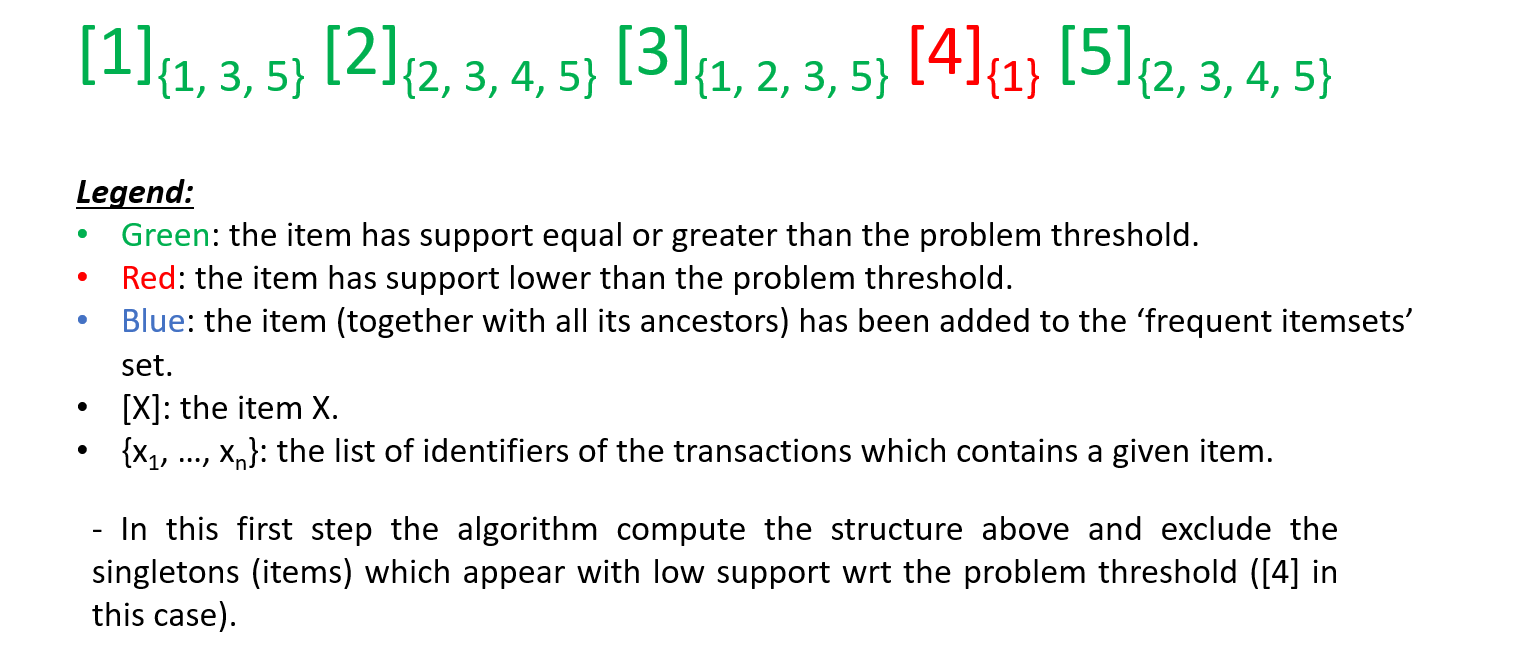
\includegraphics[scale=0.5]{./img/alg1}}

	\centerline{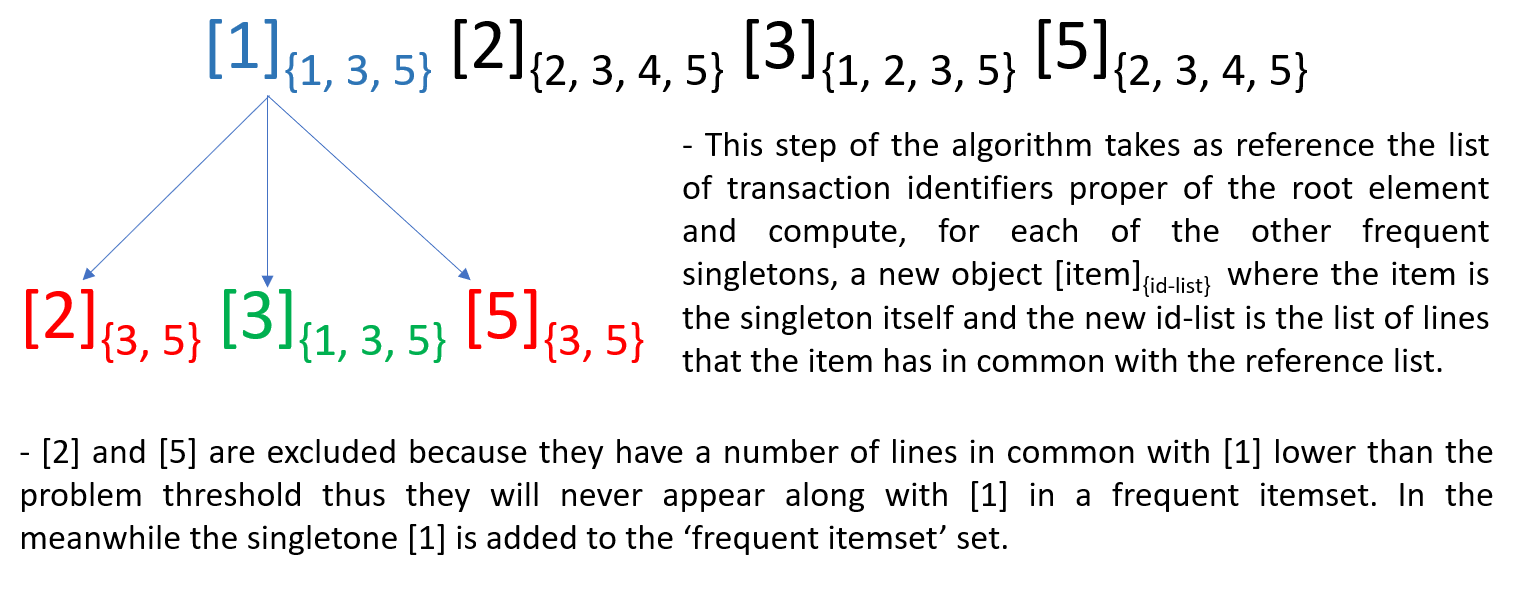
\includegraphics[scale=0.5]{./img/alg2}}
	
	\rule{\textwidth}{0.4pt}
	\\\\
	\centerline{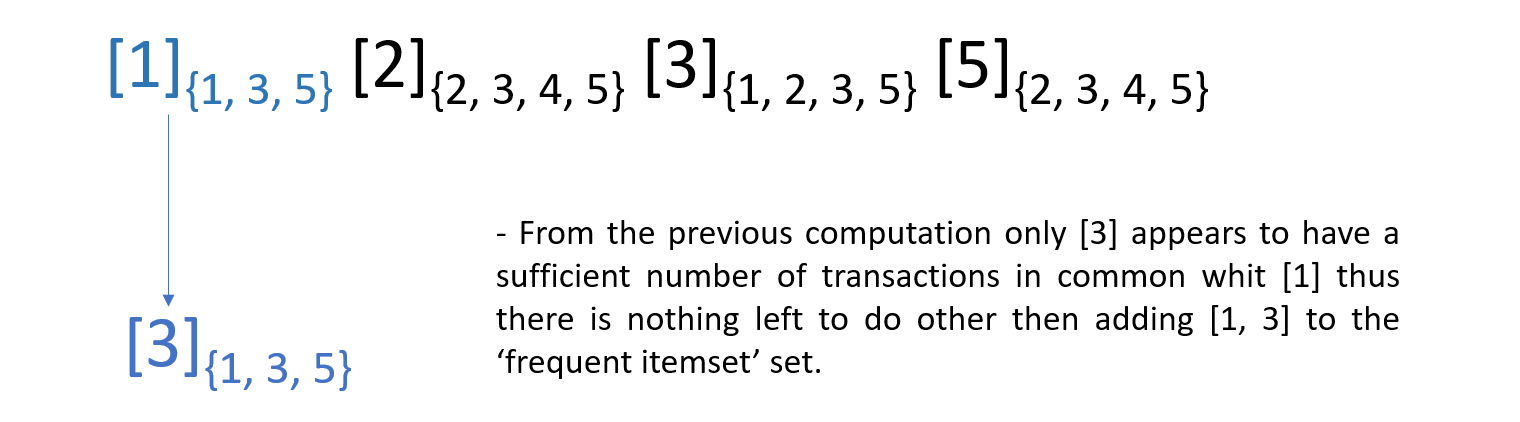
\includegraphics[scale=0.5]{./img/alg3}}
	\\\\
	\rule{\textwidth}{0.4pt}
	\\\\
	\centerline{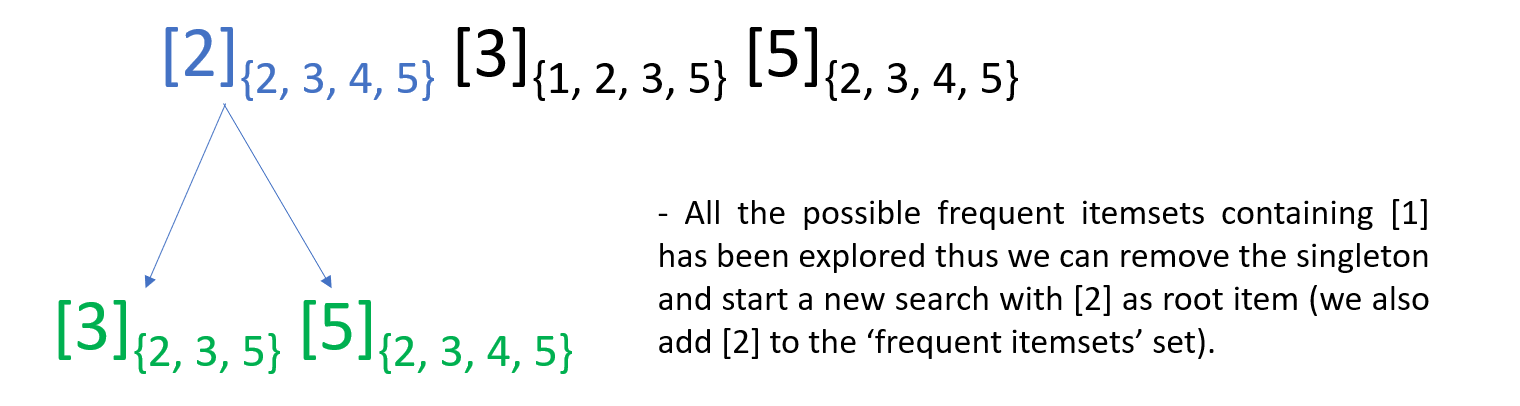
\includegraphics[scale=0.5]{./img/alg4}}
	\\\\
	\rule{\textwidth}{0.4pt}
	\\\\
	\centerline{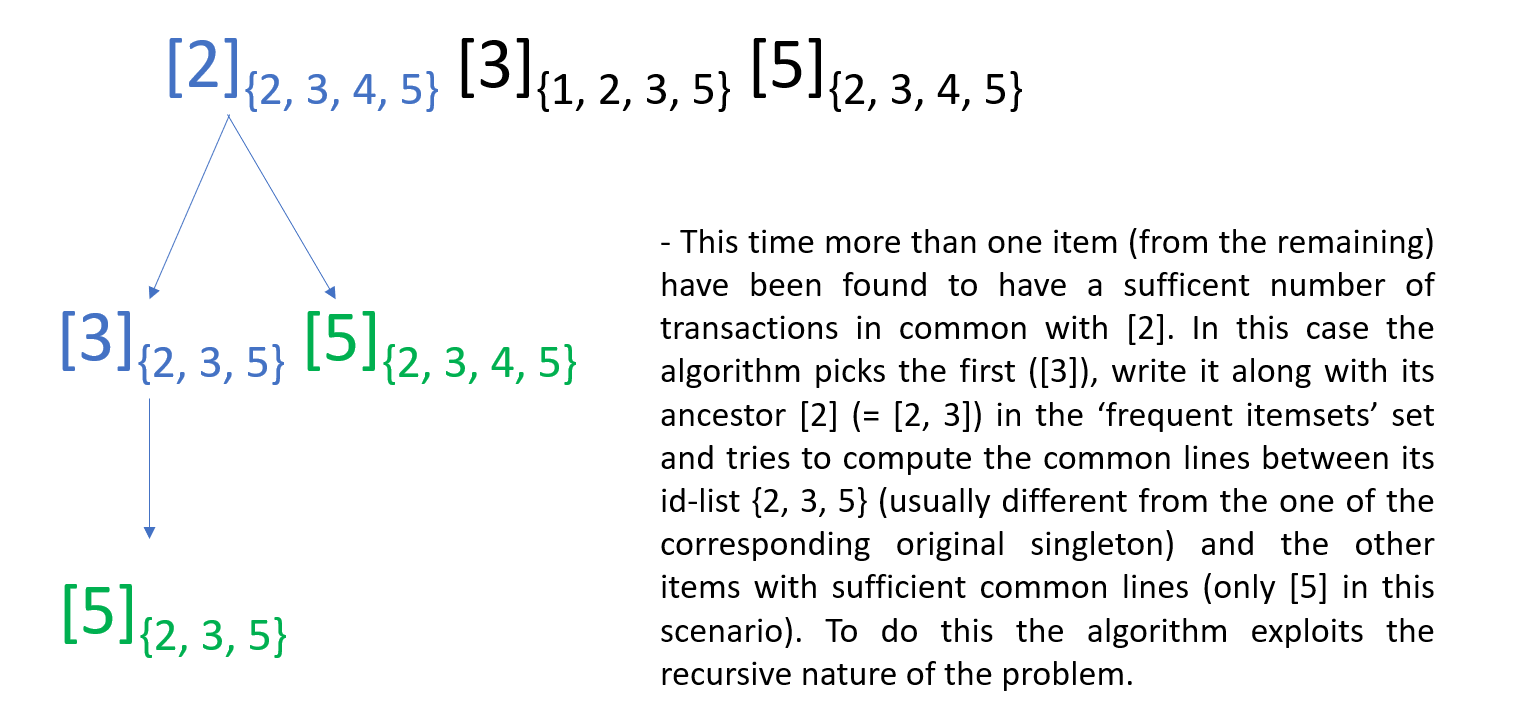
\includegraphics[scale=0.5]{./img/alg5}}

	\centerline{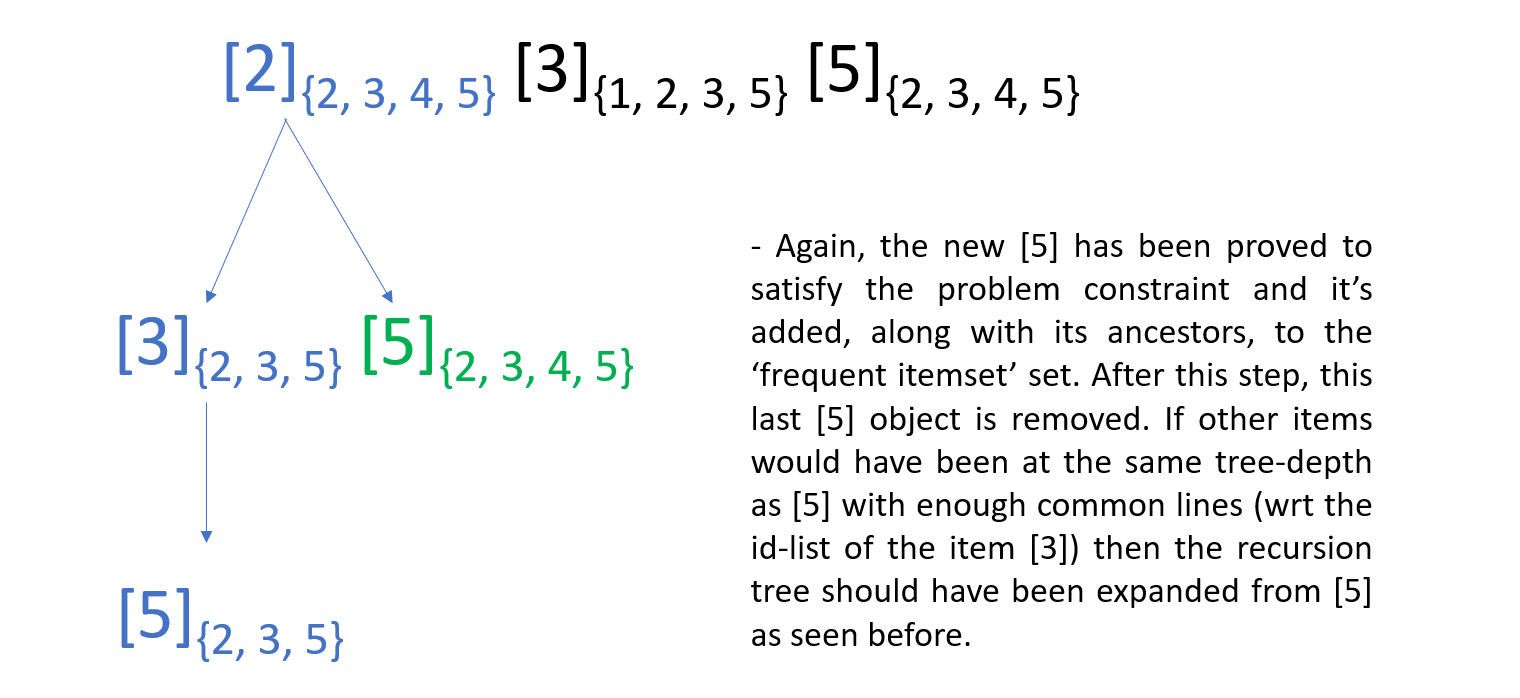
\includegraphics[scale=0.5]{./img/alg6}}
	
	\rule{\textwidth}{0.4pt}
	\\\\
	\centerline{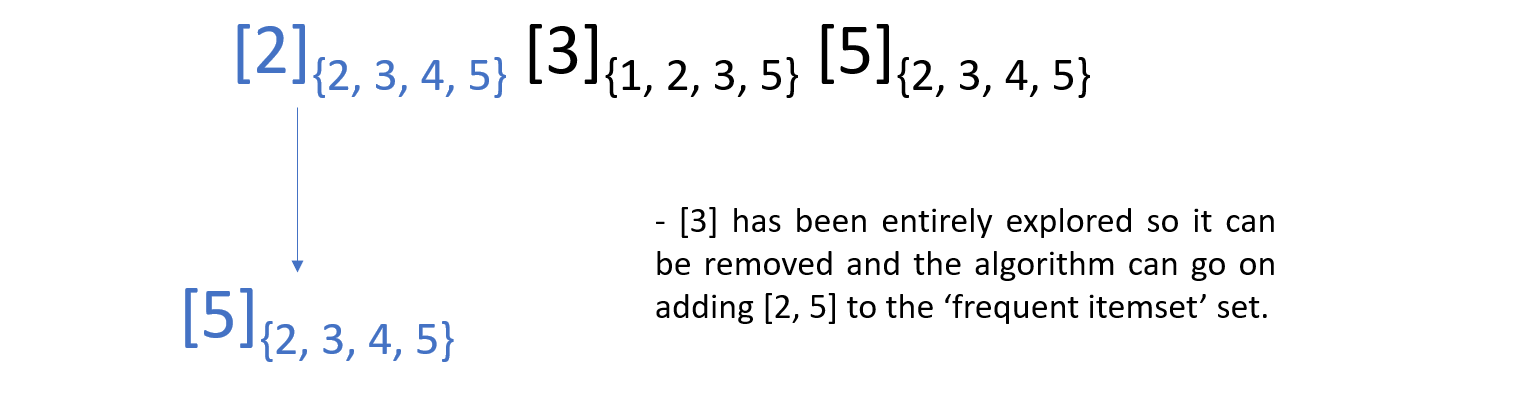
\includegraphics[scale=0.5]{./img/alg7}}
	\\\\
	\rule{\textwidth}{0.4pt}
	\\\\
	\centerline{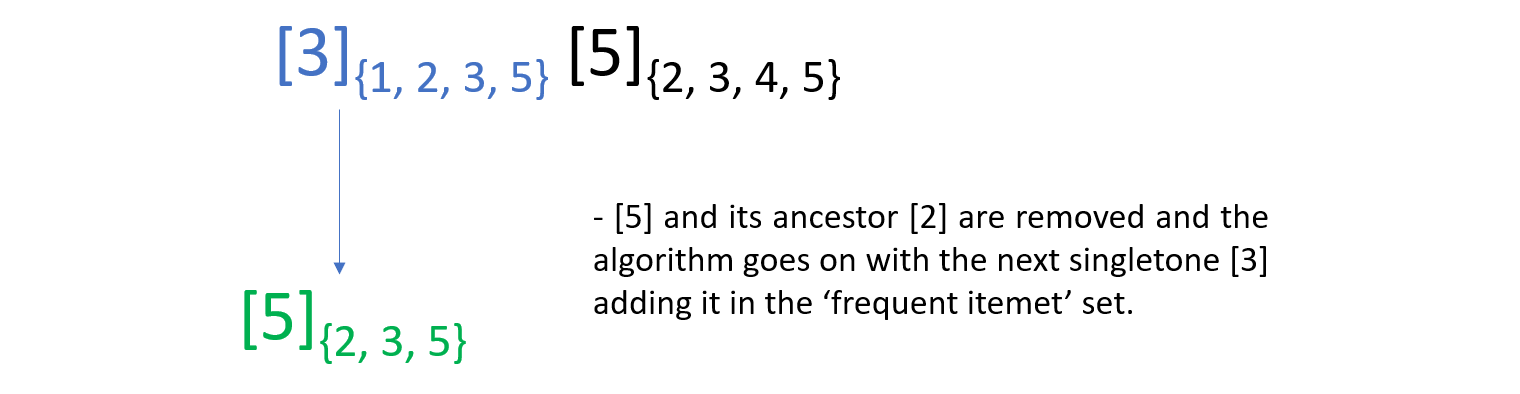
\includegraphics[scale=0.5]{./img/alg8}}
	\\\\
	\rule{\textwidth}{0.4pt}
	\\\\
	\centerline{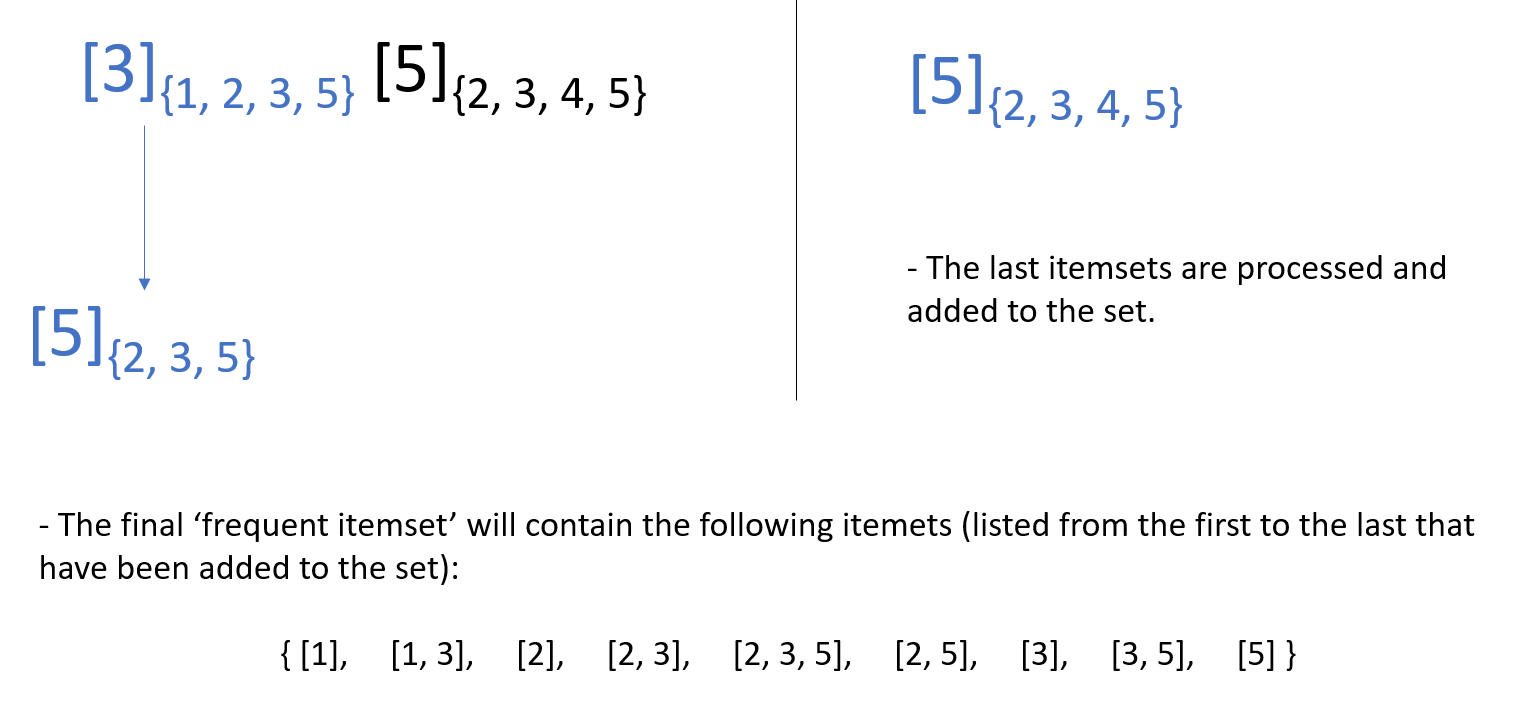
\includegraphics[scale=0.5]{./img/alg9}}
	\\
	Let's suppose now that our dataset has the following dimensions:
	\begin{itemize}
		\item \textit{Dataset total items:} M; 
		\item \textit{Singletons:} S;
		\item \textit{Occurences of the most common singleton:} K;
		\item \textit{Size of the biggest freqent itemset:} F.
	\end{itemize}
	In order to build the first singletons structure the algorithm takes \textit{\textbf{O}}(M+S) steps because, basically, it has to add to an hash-map each new singleton (key) and insert an element in a identifiers-list (value) each time a new item in the dataset is read. The following 'not-frequent singletons removal' step takes \textit{\textbf{O}}(S): it's enough to check the size of each array-list in the hash-map.  \\
	The complexity of the subsequent recursive step it's greatly influenced by the number of frequent itemsets in the datasets. In the worst case we have that all the possible itemsets are frequent thus, the algorithm will roughly perform 2$^S$  comparison between two array-lists: the reference-list (ordered) and the array-list of the item we want to add to the current frequent itemset (associated with the reference-list). This operation (comprehensive of the comparison and ignoring the faster ordering step) it's in \textit{\textbf{O}}(2$^S$*K$^2$). The complexity of this phase makes it clear that the algorithm, in order to be used, must receive as input a threshold value (\textbf{-t}) which is able to trigger a sufficient number of "cut" to the recursion tree so that it won't be completely expanded. Unfortunately this value depends on the data distribution and cannot be determined in advance.\\
	If we consider the memory usage we can state, right away, that the algorithm need at least enough space to store the whole dataset. The first structure of singletons and their lists can be seen, in fact, as a different representation of the dataset itself. In the worst case scenario all singletons will survive to the filtering step and the algorithm will begin the extraction phase with all the dataset in main memory. The recursion tree is explored with a DFS approach and the algorithm keeps in memory all the important data needed to make this recursion possible (and to speed-up the process) such as: 
	\begin{itemize}
		\item the lists of candidates items which are offspring, in the recursion tree, wrt one of the items find to be part of current frequent itemset;
		\item the hash-maps, computed at each new expansion, containing as keys the items of a specific offspring-list mentioned above and as value the common-lines list computed wrt the proper item in the recursion tree.
	\end{itemize}
	That being said it's clear that the algorithm is consuming the maximum amount of memory when the recursion tree descend its longest branch (whose element correspond to the items in the longest frequent itemset). In the worst scenario we will consume about (F/2)-time the space needed for store the dataset and (F/2)-time the space needed to store the singletons list. Unlike what we saw for the computational complexity, change the problem threshold parameter it's pointless because the memory load depend entirely on the dataset content. By the way it is still possible to reduce the memory usage by setting a maximum-size for the frequent itemsets we are looking for (thanks to the proper parameter \textbf{-m}). It's also possible to set the size of the dataset sample that each mapper will analyze (\textbf{-c}) decreasing, at least locally, the memory needed by the algorithm.          

\section*{Code Analysis:}

	This section will provide a more detailed documentation of the project classes included in 'org.myproj' package. \textit{Test.java} class won't be discuss here because beyond the focus of this report. All the information needed to use \textit{Test.java} are displayed in its command-line interface.  
	
	\subsection*{SON.java}
	This is the core class of the project, it contains the main method and represents the driver class of the whole MapReduce algorithm. In order to be executed in a MapReduce environment it extends the Hadoop class Configured and implements Tool interface.
	
	\subsubsection*{\textit{\textbf{-} Fields}} 
	This class contains a lot of fields which are listed below:
	\begin{itemize}
		\item \textit{\textbf{private double minSupp:}} support threshold parameter of the problem express either as fraction or in number of transactions;
		\item \textit{\textbf{private long numLines:}} size of the input dataset (filtered) in number of transactions (=lines); 
		\item \textit{\textbf{private long chunkSize:}} desired size of the dataset samples (in number of transactions) which will be sent to each mapper;
		\item \textit{\textbf{private MRUtil mru:}} utility class object;
		\item \textit{\textbf{private String candPath:}} HDFS path where the candidates itemsets will be stored;
		\item \textit{\textbf{private static String msg1:}} parameters-info message;
		\item \textit{\textbf{private static String msg2:}} error message to display if the filtering-job fails;
		\item \textit{\textbf{private static String msg3:}} error message to display if the first extraction-job fails; 
		\item \textit{\textbf{private static String msg4:}} error message to display if the last job fails.	
	\end{itemize}

	\subsubsection*{\textit{\textbf{-} public static void main(String[] args) throws Exception}}
	The method has the main goal to launch sequentially the three MR jobs and, eventually, display the proper error message. It also calls the \textit{readArgs} in order to parse its raw input parameters.  
	\begin{description}
		\item - Input:
		\begin{itemize}
			\item \textit{args:} list of arguments from command line.
		\end{itemize}
	\end{description}
	\begin{description}
		\item - Output:
		\begin{itemize}
			\item \textit{none} 
		\end{itemize}
	\end{description}

	\subsubsection*{\textit{\textbf{-} public SON(String[] args, MRUtil mru)}}
		Class constructor which simply initialize \textbf{minSupp}, \textbf{chunkSize} and \textbf{mru} fields.  
	\begin{description}
		\item - Input:
		\begin{itemize}
			\item \textit{args:} list of arguments parsed and ready to be used;
			\item \textit{mru:} utility class object.
		\end{itemize}
	\end{description}
   
	\subsubsection*{\textit{\textbf{-} private static void error(String uri, String tmp, String msg) throws IllegalArgumentException, IOException}}
	Private utility method used to send messages to standard error and clean \textit{tmp} directory from HDFS. In order to complete this last task an utility class is used.  
	\begin{description}
		\item - Input:
		\begin{itemize}
			\item \textit{uri:} cluster URI used to access HDFS;
			\item \textit{tmp:} path of the directory we want to remove;
			\item \textit{msg:} error message.
		\end{itemize}
	\end{description}
	\begin{description}
		\item - Output:
		\begin{itemize}
			\item \textit{none} 
		\end{itemize}
	\end{description}	
	 
	\subsubsection*{\textit{\textbf{-} public int run(String[] argsRun) throws Exception}}   	
  	This method overrides the \textit{run} method in Tool interface. It creates a new Job instance and configures it thanks to the utility class MRUtil. This method is responsible for the configuration of all three MR jobs and also for the initialization of the two fields \textbf{numLines} and \textbf{chunkSize} which can be initialize only after the end of the filtering job. In particular \textbf{chunkSize} is initialized only if its value is negative (a specific chunk size has not been submitted from command line).  
	\begin{description}
		\item - Input:
		\begin{itemize}
			\item \textit{argsRun:} list of arguments parsed and ready to be used.
		\end{itemize}
	\end{description}
	\begin{description}
		\item - Output:
		\begin{itemize}
			\item \textit{i:} int value, if \textit{i}=0 state that the job is ended as expected (otherwise its value will be 1). 
		\end{itemize}
	\end{description}
	\vskip 20pt
	\subsection*{MRSUtil.java}
	This class contains some supplementary methods related to the configuration of the map-reduce environment. This class has not a specific role: it has been used mainly to enhance code readability.
	
	\subsubsection*{\textit{\textbf{-} Fields}} 
	Here we have only the following field:
	\begin{itemize}
		\item \textit{\textbf{private Configuration conf:}} configuration object which is used by several class methods. 
	\end{itemize}

	\subsubsection*{\textit{\textbf{-} private Job config(String name, \\
			       Class<? extends Mapper> clMap,\\ 
			       Class<? extends Reducer> clRed,\\
			       Class<?> mOutK, \\
			       Class<?> mOutV,\\
			       Class<? extends InputFormat> informat,\\ 
			       Class<? extends OutputFormat> outformat,\\
			       String pathin,\\
			       String pathout) throws IOException}}   	
	This method is used to set up the Configuration object instance represented by the class field \textbf{conf}. It's a private method called by each one of the three public methods below that are specific for each job. This method has a lot of input parameters: these are necessary to configure the job <key,value> pairs type, the InputFormat and OutputFormat classes, the input and output file/directory of the job and the Mapper and Reducer classes to use.    
	\begin{description}
		\item - Input:
		\begin{itemize}
			\item \textit{name:} name of the job;
			\item \textit{clMap:} Mapper class;
			\item \textit{clRed:} Reducer class;
			\item \textit{mOutK:} class of the keys genereted (in the output pairs) by the Mapper;
			\item \textit{mOutV:}class of the values generated (in the output pairs) by the Mapper;
			\item \textit{informat:} InputFormat class;
			\item \textit{outformat:} OutputFormat class;
			\item \textit{pathin:} input path;
			\item \textit{pathout:} output path.
		\end{itemize}
	\end{description}
	\begin{description}
		\item - Output:
		\begin{itemize}
			\item \textit{job:} the brand new Job instance just generated. 
		\end{itemize}
	\end{description}
	
	\subsubsection*{\textit{\textbf{-} public Job configFilter(Configuration conf, String[] args) throws IOException }}   	
	This method is used to set up the configuration of the filtering job. The configuration will have \textit{FilterMap} as Mapper class and \textit{FilterReduce} as Reducer class. The Mapper class will emit Text objects as keys and LongWritable as values. Both Input and Output format are set to \textit{TextInputFormat/TextOutputFormat}. All these information (along with the number of reducers) are retrieved by the input argument \textit{args}.
	\begin{description}
		\item - Input:
		\begin{itemize}
			\item \textit{conf:} configuration to set up;
			\item \textit{args:} list of arguments used to configure the job.
		\end{itemize}
	\end{description}
	\begin{description}
		\item - Output:
		\begin{itemize}
			\item \textit{job:} the new Job instance. 
		\end{itemize}
	\end{description}
	
	\subsubsection*{\textit{\textbf{-} 	public Job configFirst(Configuration conf, String[] args, long numLines) throws IOException}}   	
	Like the previous method, its role is to configure a new job related, this time, to the first MR extraction cycle. The differences here are that Mapper and Reducer classes are now \textit{FirstMap} and \textit{FirstReduce}.  The InputFormat class is now the custom \textit{MultilineInputFormat} class which extends NLineInputFormat and requires, for this reason, a new parameter: the number of lines per split. For this job two additional configuration fields are generated: one will contain the number of transactions of the entire dataset and the other the max-size of the frequent itemsets(/candidates) we want to find.
	\begin{description}
		\item - Input:
		\begin{itemize}
			\item \textit{conf:} configuration to set up;
			\item \textit{args:} list of arguments used to configure the job;
			\item \textit{numLines:} total number of transactions in the datasets.
		\end{itemize}
	\end{description}
	\begin{description}
		\item - Output:
		\begin{itemize}
			\item \textit{job:} the new Job instance. 
		\end{itemize}
	\end{description}	
	
	\subsubsection*{\textit{\textbf{-} public Job configSecond(Configuration conf, String[] args, long numLines, String cp) throws IOException }}   	
	This method is very similar to the previous except for the two MR classes which are now \textit{SecondMap} and \textit{secondReduce}. Some other fields are added to the configuration by this method: these are the cluster URI, the HDFS directory where to find the output of the previous job and, again, the number of transactions of the dataset. The remaining configuration parameters are the same seen before.  
	\begin{description}
		\item - Input:
		\begin{itemize}
			\item \textit{conf:} configuration to set up;
			\item \textit{args:} list of arguments used to configure the job;
			\item \textit{numLines:} total number of transactions in the datasets;
			\item \textit{cp:}.
		\end{itemize}
	\end{description}
	\begin{description}
		\item - Output:
		\begin{itemize}
			\item \textit{job:} the new Job instance. 
		\end{itemize}
	\end{description}

	\subsubsection*{\textit{\textbf{-} public void setMinSupp(Job job, double minSupp)}}   	
	We use this method to set up the configuration fields related to the problem support threshold. These are two values: a boolean, which state if the support has been submitted as fraction or not, and the proper Double or Long field related to the actual threshold value.    
	\begin{description}
		\item - Input:
		\begin{itemize}
			\item \textit{job:} the Job instance whose configuration will be updated;
			\item \textit{minSupp:} the threshold value.
		\end{itemize}
	\end{description}
	\begin{description}
		\item - Output:
		\begin{itemize}
			\item \textit{none} 
		\end{itemize}
	\end{description}

	\subsubsection*{\textit{\textbf{-} public String[] readArgs(String[] args)}}   	
	This method is responsible for the interpretation of the optional command-line arguments. It returns a new list of arguments which contains all the necessary values.  
	\begin{description}
		\item - Input:
		\begin{itemize}
			\item \textit{args:} the command-line arguments.
		\end{itemize}
	\end{description}
	\begin{description}
		\item - Output:
		\begin{itemize}
			\item \textit{newargs:} the new arguments ready to be used. 
		\end{itemize}
	\end{description}

	
	\subsection*{HDFSUtil.java}
	This class implements the methods needed by the algorithm to interact with HDFS.
	\subsubsection*{\textit{\textbf{-} Fields}} 
	The class contains the following fields:
	\begin{itemize}
		\item \textit{\textbf{private String uri:}} URI of the HDFS cluster;
		\item \textit{\textbf{private String file:}} last file read by the class;
		\item \textit{\textbf{private int offset:}} file offset; 
		\item \textit{\textbf{private boolean hasnext:}} state if the file contains unread lines;		
	\end{itemize}

	\subsubsection*{\textit{\textbf{-} public HDFSUtil(String uri)}}   	
	This is the constructor of the class which simply set up the \textbf{uri} field.   
	\begin{description}
		\item - Input:
		\begin{itemize}
			\item \textit{uri:} URI of the HDFS cluster.
		\end{itemize}
	\end{description}


	\subsubsection*{\textit{\textbf{-} public void deleteDir(Path dir) throws IOException}}   	
	This method delete the HDFS directory (and its content) whose path is specified as input parameter.
	\begin{description}
		\item - Input:
		\begin{itemize}
			\item \textit{dir:} HDFS directory path;
		\end{itemize}
	\end{description}
	\begin{description}
		\item - Output:
		\begin{itemize}
			\item \textit{none} 
		\end{itemize}
	\end{description}


	\subsubsection*{\textit{\textbf{-} public ArrayList<String> dirFiles(String dir) throws IOException}}   	
	This method return the list of files in the HDFS directory whose path is specified as input.
	\begin{description}
		\item - Input:
		\begin{itemize}
			\item \textit{dir:} HDFS directory path.
		\end{itemize}
	\end{description}
	\begin{description}
		\item - Output:
		\begin{itemize}
			\item \textit{files:} list of HDFS file names (comprehensive of file paths). 
		\end{itemize}
	\end{description}


	\subsubsection*{\textit{\textbf{-} public ArrayList<List<Long>$>$ readCands(String cndf, int lines) throws IOException}}   	
	This method is used to read the candidates itemsets written in a file. In order to do this, the method reads a chunk of the file (starting from the current offset) and then it parses the chunk extracting a list of Long values (candidate itemset) from each line. 
	\begin{description}
		\item - Input:
		\begin{itemize}
			\item \textit{cnfd:} HDFS file path;
			\item \textit{lines:} max number of lines to read. 
		\end{itemize}
	\end{description}
	\begin{description}
		\item - Output:
		\begin{itemize}
			\item \textit{cands:} ArrayList of candidates; each one of them is represented as list of Long values. 
		\end{itemize}
	\end{description}


	\subsubsection*{\textit{\textbf{-} private String readFile(String filepath, int lines) throws IOException}}   	
	This private method is responsible of reading a chunk of the file whose path is given as input (along with the size of the chunk to read). In order to do this, the method opens a connection with the cluster HDFS and then opens an input stream related to the desired file. The function exploit the class field \textbf{offset} to skip the unwanted lines of the file.    
	\begin{description}
		\item - Input:
		\begin{itemize}
			\item \textit{filepath:} path of the file to read;
			\item \textit{lines:} max number of lines to read.
		\end{itemize}
	\end{description}
	\begin{description}
		\item - Output:
		\begin{itemize}
			\item \textit{s:} the file chunk. 
		\end{itemize}
	\end{description}

	\subsubsection*{\textit{\textbf{-} public boolean hasNext(String cndf)}}   	
	This method states if the file (whose path is given as input) contains unread lines. If the file path is different than the current it returns true.  
	\begin{description}
		\item - Input:
		\begin{itemize}
			\item \textit{cndf:} file path;
		\end{itemize}
	\end{description}
	\begin{description}
		\item - Output:
		\begin{itemize}
			\item \textit{(boolean):} true if the file contains unread lines, false otherwise. 
		\end{itemize}
	\end{description}
	
	\rule{\textwidth}{0.4pt}
	
	
	\subsection*{FilterMR.java: FilterMap Class}
	
	This class extend the hadoop class Mapper and it's used, in fact, as Mapper class for the filtering job. Its role is to read the input dataset line by line and parse each one of them. 
	
	\subsubsection*{\textit{\textbf{-} Fields}} 
	The class has the following fields:
	\begin{itemize}
		\item \textit{\textbf{private Text k:}} Text object used to temporary store a key;
		\item \textit{\textbf{private LongWritable v:}} LongWritable object used to temporary store a value; 
	\end{itemize}
	
	\subsubsection*{\textit{\textbf{-} protected void map(LongWritable key, Text value, Context context) throws IOException, InterruptedException}}   	
	This is the map method used in the MR cycle whose role is to read each line of the dataset, extract the transaction id and the item from the current line (input value) and emit them as a <key,value> pair with format specified in the header.  
	\begin{description}
		\item - Input:
		\begin{itemize}
			\item \textit{key:} LongWritable representing the offset of the dataset file;
			\item \textit{value:} Text containing the current line;
			\item \textit{context:} Context instance used to "write"(emit) the pairs.
		\end{itemize}
	\end{description}
	\begin{description}
		\item - Output:
		\begin{itemize}
			\item \textit{none} 
		\end{itemize}
	\end{description}
	
	\subsection*{FilterMR.java: FilterReduce Class}
	This class represents the Reducer for the filtering job.
	\subsubsection*{\textit{\textbf{-} Fields}} 
	The class has the following fields:
	\begin{itemize}
		\item \textit{\textbf{private Text k:}} Text object used to temporary store a key;
		\item \textit{\textbf{private static Text v:}} Text static fields: it will be the value for all the output pairs.
	\end{itemize}
	
	\subsubsection*{\textit{\textbf{-} 	protected void reduce(Text trs, Iterable<LongWritable> items, Context context) throws IOException, InterruptedException}}   	
	This is the reduce method used in the filtering job. It receives as input a transaction-id (key) and all the items related to that id. Its main goal is to re-format this collection of items in a string and emits it as Text key along with an "empty" value.     
	\begin{description}
		\item - Input:
		\begin{itemize}
			\item \textit{trs:} Text key representing the transaction identifier;
			\item \textit{items:} collection of items related to the current key;
			\item \textit{context:} Context instance used to "write"(emit) the pairs.
		\end{itemize}
	\end{description}	
	\begin{description}
		\item - Output:
		\begin{itemize}
			\item \textit{none} 
		\end{itemize}
	\end{description}
	
	\rule{\textwidth}{0.4pt}

		
	\subsection*{MultilineInputRecord.java}
	This class implements the custom InputFormat class needed to read the dataset chunk by chunk. It extends NLineInputFormat whose methods ensure that the split offset that each one of the custom RecordReader will receive, will point to a valid line. A valid line must have as line-offset a multiple of the class parameter \textit{linespermap} set during the configuration step. Such class is required by the framework if we want to use a custom RecordReader.    
	
	\subsubsection*{\textit{\textbf{-} Fields}} 
	This class has no-additional fields wrt the class it extends.
	
	\subsubsection*{\textit{\textbf{-} 	public RecordReader<LongWritable, Text> createRecordReader(InputSplit genericSplit, TaskAttemptContext context)}}   	
	This method is used to create a record reader for a given split. The framework will call \textit{RecordReader.initialize(InputSplit, TaskAttemptContext)} before the split is used.   
	\begin{description}
		\item - Input:
		\begin{itemize}
			\item \textit{genericSplit:} the split to be read;
			\item \textit{context:} the context containing the information about the task.
		\end{itemize}
	\end{description}	
	\begin{description}
		\item - Output:
		\begin{itemize}
			\item \textit{(MultiLineRecordReader):} a new instance of the custom record reader. 
		\end{itemize}
	\end{description}
	
	\rule{\textwidth}{0.4pt}
	
	\subsection*{MultiLineRecordReader.java}
	This class extends the Hadoop class RecordReader which is responsible for the extraction of the <key,value> pairs from the files splits. The pairs produced by this class will have a LongWritable object as key and a Text object as value. In particular, the Text object will be generated starting from a String which represent the entire file split. Occasionally this String could include all the text of the successive split if this one has less line than expected. In this case the successive split will be skipped (this could happen at the end of a file). 
	
	\subsubsection*{\textit{\textbf{-} Fields}} 
	The class contains the following fields:
	\begin{itemize}
		\item \textit{\textbf{private LongWritable key:}} key to set and return when required;
		\item \textit{\textbf{private Text value:}} value to set and return when required;
		\item \textit{\textbf{private LineReader in:}} instance of the class LineReader used to read from input stream; 
		\item \textit{\textbf{private long start:}} offset which represent the beginning of the split;
		\item \textit{\textbf{private long end:}} offset of the end of the split;
		\item \textit{\textbf{private long pos:}} current offset;
		\item \textit{\textbf{private int nlines:}} number of lines expected to be part of a split.	
	\end{itemize}

	\subsubsection*{\textit{\textbf{-} public void close() throws IOException}}   	
	This method close the input stream reader \textbf{in}.    
	\begin{description}
		\item - Input:
		\begin{itemize}
			\item \textit{none}
		\end{itemize}
	\end{description}	
	\begin{description}
		\item - Output:
		\begin{itemize}
			\item \textit{none} 
		\end{itemize}
	\end{description}

	\subsubsection*{\textit{\textbf{-} public LongWritable getCurrentKey() throws IOException, InterruptedException}}   	
	This method return the last key that has been read.   
	\begin{description}
		\item - Input:
		\begin{itemize}
			\item \textit{none}
		\end{itemize}
	\end{description}	
	\begin{description}
		\item - Output:
		\begin{itemize}
			\item \textit{key}: the class field described above. 
		\end{itemize}
	\end{description}

	\subsubsection*{\textit{\textbf{-} public Text getCurrentValue() throws IOException, InterruptedException}}   	
	This method return the last value that has been read.    
	\begin{description}
		\item - Input:
		\begin{itemize}
			\item \textit{none}
		\end{itemize}
	\end{description}	
	\begin{description}
		\item - Output:
		\begin{itemize}
			\item \textit{value:} the class field described above.  
		\end{itemize}
	\end{description}

	\subsubsection*{\textit{\textbf{-} public float getProgress() throws IOException, InterruptedException}}   	
	This method return a float number between 0 and 1 representing the fraction of the split that has been processed. 
	\begin{description}
		\item - Input:
		\begin{itemize}
			\item \textit{none}
		\end{itemize}
	\end{description}	
	\begin{description}
		\item - Output:
		\begin{itemize}
			\item \textit{(float):} the progress value. 
		\end{itemize}
	\end{description}

	\subsubsection*{\textit{\textbf{-} public void initialize(InputSplit genericsplit, TaskAttemptContext context) throws IOException, InterruptedException}}   	
	With this method we initialize the main fields of the class. These are the \textbf{start}, \textbf{end}, \textbf{pos}, and \textbf{in} fields. In particular, the value of \textbf{pos} is set to be equal to \textbf{start}. This last field value could change during the execution depending on the fact that the split is or is not at the beginning of the file (\textbf{start}=0). In fact, this method is intended to skip a line (after backtracking of the offset) if \textbf{start}$\neq$0: this is done to avoid reading two time the same line whenever the previous split had a last line which surpass its end offset. In this scenario \textbf{start} is set at the beginning of the first unread line.   
	\begin{description}
		\item - Input:
		\begin{itemize}
			\item \textit{genericsplit:} the split to parse;
			\item \textit{context:} the context which contains information about the current job.
		\end{itemize}
	\end{description}	
	\begin{description}
		\item - Output:
		\begin{itemize}
			\item \textit{none}  
		\end{itemize}
	\end{description}

	\subsubsection*{\textit{\textbf{-} public boolean nextKeyValue() throws IOException, InterruptedException}}   	
	This method updates the \textbf{key} and \textbf{value} fields and states if there is a pair ready to be read (= if key and value have been updated or not). This method also try to read the lines of the next split: if they are less tan the expected number then they are added to the current value. This is to prevent the algorithm to read chunks too small (could cause problems when scaling the support threshold).   
	\begin{description}
		\item - Input:
		\begin{itemize}
			\item \textit{none}
		\end{itemize}
	\end{description}	
	\begin{description}
		\item - Output:
		\begin{itemize}
			\item \textit{(boolean):} true if the split is bigger then the file (the file has been completely read) or if the correct amount of line has been read. 
		\end{itemize}
	\end{description}	
	
	\rule{\textwidth}{0.4pt}
	
	\subsection*{FQItemset.java}
	This is the class responsible for frequent itemsets extraction. Its behavior has been explained in the last section.
	
	\subsubsection*{\textit{\textbf{-} Fields}} 
	The class fields are the following:
	\begin{itemize}
		\item \textit{\textbf{private long minsupp:}} problem support threshold expressed in number of transactions;
		\item \textit{\textbf{private List<Long> actual:}} current frequent itemset;
		\item \textit{\textbf{private ArrayList<String> freq:}} list of frequent itemsets expressed as string;
		\item \textit{\textbf{private HashMap<Long,List<Long>> idxs:}} HasMap used to store the singletons as keys and their corresponding list of transactions identifiers as value;
		\item \textit{\textbf{private long maxitms:}} the max length of the frequent itemsets we are looking for;
		\item \textit{\textbf{private Context context:}} necessary in order to emit pairs when used in a MR job; 		 
		\item \textit{\textbf{private LongWritable v:}} LongWritable object used as value whenever a <key, value> pair needs to be written.	
	\end{itemize}
	
	\subsubsection*{\textit{\textbf{-} public FQItemset(String[] lines, long minsupp, long maxitms)}}   	
	This is the class constructor used to test the class in a standard environment. It simply delegates the class initialization to the proper private method.
	   
	\begin{description}
		\item - Input:
		\begin{itemize}
			\item \textit{lines:} list of dataset transactions each one expressed as String;
			\item \textit{minsupp:} support threshold in number of transactions;
			\item \textit{maxitms:}  the max length of the frequent itemsets.
		\end{itemize}
	\end{description}
	
	\subsubsection*{\textit{\textbf{-} public FQItemset(String[] lines, long minsupp, long maxitms, Context context)}}   	
	This is the class constructor used in the proper MR jobs. It delegates the class initialization to the proper private method and initialize the class field \textbf{context}.    
	\begin{description}
		\item - Input:
		\begin{itemize}
			\item \textit{lines:} list of dataset transactions each one expressed as String;
			\item \textit{minsupp:} support threshold in number of transactions;
			\item \textit{maxitms:} the max length of the frequent itemsets;
			\item \textit{context:} received from a Mapper, it's necessary in order to emit pairs when used in a MR job.
		\end{itemize}
	\end{description}

	\subsubsection*{\textit{\textbf{-} private void FQItemsetIni(String[] lines, long minsupp, long maxitms)}}   	
	This method initializes the main fields of the class. In particular, \textbf{minsupp} and \textbf{maxitms} are set thanks to the namesakes input parameters. Instead, \textbf{idxs} is built singleton by singleton parsing the input array \textit{lines}. When the hashmap is completed it has to be filtered by the proper method to remove the non-frequent singletons.   
	\begin{description}
		\item - Input:
		\begin{itemize}
			\item \textit{lines:} list of dataset transactions each one expressed as String;
			\item \textit{minsupp:} support threshold in number of transactions;
			\item \textit{maxitms:} the max length of the frequent itemsets;
		\end{itemize}
	\end{description}	
	\begin{description}
		\item - Output:
		\begin{itemize}
			\item \textit{none}  
		\end{itemize}
	\end{description}
	
	\subsubsection*{\textit{\textbf{-} public ArrayList<String> findFrequent() throws IOException, InterruptedException}}   	
	Header method whose role is to start the recursive algorithm used to extract the frequent itemsets which contain the first key in \textbf{idxs}.    
	\begin{description}
		\item - Input:
		\begin{itemize}
			\item \textit{none}
		\end{itemize}
	\end{description}	
	\begin{description}
		\item - Output:
		\begin{itemize}
			\item \textit{freq:} the class field which can be either the list of frequent itemsets (standard environment) or an empty list (MR environment: \textbf{context}$\neq$$null$). 
		\end{itemize}
	\end{description}
	
	\subsubsection*{\textit{\textbf{-} private void findFrequentRecursive(HashMap<Long,List<Long>> idxs, long count) throws IOException, InterruptedException}}   	
	This method adds an other element to the current frequent itemset stored in \textbf{actual} field: this item is the first in the local hashmap \textit{idxs}. The method calls the private function \textit{parseFreq} and then computes a new hashmap of the items that have enough transactions in common with the current frequent itemset in \textbf{actual}. After this, the method proceeds with a recursive call (for each element in \textit{idxs}) passing as input values the new hashmap and the new incremented depth value.   
	  
	\begin{description}
		\item - Input:
		\begin{itemize}
			\item \textit{idxs:} new HashMap of items (and their occurrences) who have been proven to be part of a frequent itemset;
			\item \textit{count:} current recursion tree depth.
		\end{itemize}
	\end{description}	
	\begin{description}
		\item - Output:
		\begin{itemize}
			\item \textit{none} 
		\end{itemize}
	\end{description}
	
	\subsubsection*{\textit{\textbf{-} private ArrayList<Long> commonLines(List<Long> first, List<Long> second)}}   	
	This method takes as input two List of Long values and return the list of common values between the two.    
	\begin{description}
		\item - Input:
		\begin{itemize}
			\item \textit{first:} first input list;
			\item \textit{second:} second input list.
		\end{itemize}
	\end{description}	
	\begin{description}
		\item - Output:
		\begin{itemize}
			\item \textit{common:} list of common Long values. 
		\end{itemize}
	\end{description}
	
	\subsubsection*{\textit{\textbf{-} private void rmSingletones()}}   	
	This private method has the goal to filter the hashmap \textbf{idxs} removing the singletons that don't appear in enough transactions (< then \textbf{minsupp}).   
	\begin{description}
		\item - Input:
		\begin{itemize}
			\item \textit{none}
		\end{itemize}
	\end{description}	
	\begin{description}
		\item - Output:
		\begin{itemize}
			\item \textit{none} 
		\end{itemize}
	\end{description}
	
	\subsubsection*{\textit{\textbf{-} public boolean hasNext()}}   	
	This method is used to know if there are other itemsets to check.   
	\begin{description}
		\item - Input:
		\begin{itemize}
			\item \textit{none}
		\end{itemize}
	\end{description}	
	\begin{description}
		\item - Output:
		\begin{itemize}
			\item \textit{(boolean):} true if \textbf{idxs} contains other keys. 
		\end{itemize}
	\end{description}
	
	\subsubsection*{\textit{\textbf{-} public void setSingletones(ArrayList<Long> trn, long c)}}   	
	This method takes as input a transaction, expressed as list of items, and its identifier. It updates \textbf{idxs} hashmap adding the transaction-id to the lists related to each singleton which appears in the transaction. If a transaction item doesn't appear as key in the hashmap is added.    
	\begin{description}
		\item - Input:
		\begin{itemize}
			\item \textit{trn:} transaction expressed as list of Long values (items);
			\item \textit{c:} transaction identifier.
		\end{itemize}
	\end{description}	
	\begin{description}
		\item - Output:
		\begin{itemize}
			\item \textit{none} 
		\end{itemize}
	\end{description}
	
	\subsubsection*{\textit{\textbf{-} private void parseFreq(List<Long> freq) throws IOException, InterruptedException}}   	
	This method transforms a frequent itemset in a String and, depending on the presence of the class field \textbf{context}, emits a <key,value> pair or updates the list \textbf{freq}.  
	\begin{description}
		\item - Input:
		\begin{itemize}
			\item \textit{freq:} frequent itemset as list of Long values (items).
		\end{itemize}
	\end{description}	
	\begin{description}
		\item - Output:
		\begin{itemize}
			\item \textit{none} 
		\end{itemize}
	\end{description}
	
	\subsubsection*{\textit{\textbf{-} public long getCount(List<Long> cand)}}   	
	This method counts the occurrences of a given itemset. It does this by finding the transactions that are common to all the singletons in the itemset.    
	\begin{description}
		\item - Input:
		\begin{itemize}
			\item \textit{cand:} itemset as list of Long values (items).
		\end{itemize}
	\end{description}	
	\begin{description}
		\item - Output:
		\begin{itemize}
			\item \textit{(long):} number of occurrences of the given itemset. 
		\end{itemize}
	\end{description}


	\rule{\textwidth}{0.4pt}	

	\subsection*{FirstMR.java: FirstMap Class}
	This is the Mapper class that is used by the first extraction-job. 
	\subsubsection*{\textit{\textbf{-} Fields}} 
	The class contains the following fields:
	\begin{itemize}
		\item \textit{\textbf{private long numLines:}} total number of transactions in the dataset;
		\item \textit{\textbf{private boolean isFraction:}} states if the problem threshold is expressed as fraction or not;
		\item \textit{\textbf{private long minSuppL:}} stores the threshold value if it's not expressed as fraction; 
		\item \textit{\textbf{private double minSuppD:}} stores the threshold value if it's expressed as fraction;
		\item \textit{\textbf{private long maxitms:}} max length of the frequent itemsets we want.	
	\end{itemize}
	
	\subsubsection*{\textit{\textbf{-} protected void setup(Context context) throws IOException, InterruptedException}}   	
	This method initializes the class fields exploiting the input parameter \textit{context} from which is possible to obtain the job configuration and its fields.  
	\begin{description}
		\item - Input:
		\begin{itemize}
			\item \textit{context:} stores information about the current job.
		\end{itemize}
	\end{description}	
	\begin{description}
		\item - Output:
		\begin{itemize}
			\item \textit{none} 
		\end{itemize}
	\end{description}
	
	\subsubsection*{\textit{\textbf{-} protected void map(LongWritable key, Text value, Context context) throws IOException, InterruptedException}}   	
	This is the map method of the first extraction job. This method will scale the threshold parameter according to the size (in lines) of the chunk received as input. It will also divide the chunk in lines and generate an istance of the class FQItemset. Thanks to this new instance it will be possible to find the candidates itemsets and emit them as <key, value> pairs where the key will be a Text object (generated from the string representing a candidate) and the value a placeholder of class LongWritable.    
	\begin{description}
		\item - Input:
		\begin{itemize}
			\item \textit{key:} LongWritable representing the offset of the dataset file;
			\item \textit{value:} Text containing the entire chunk read by MultiLineRecordReader;
			\item \textit{context:} stores information about the current job.
		\end{itemize}
	\end{description}	
	\begin{description}
		\item - Output:
		\begin{itemize}
			\item \textit{none} 
		\end{itemize}
	\end{description}
	
	
	\subsection*{FirstMR.java: FirstReduce Class}
	This is the class used as Reducer in the first extraction-job.
	\subsubsection*{\textit{\textbf{-} Fields}} 
	The class contains the following fields:
	\begin{itemize}
		\item \textit{\textbf{private Text v:}} an "empty" Text object used as value in the output pairs of this class reduce function.	
	\end{itemize}
	
	\subsubsection*{\textit{\textbf{-} protected void reduce(Text freqitem, Iterable<LongWritable> value, Context context) throws IOException, InterruptedException}}   	
	This reduce function will simply emit a pairs for each key it receives. This pairs will be composed by the method input key as key and the field \textbf{v} as value.    
	\begin{description}
		\item - Input:
		\begin{itemize}
			\item \textit{freqitem:} Text key representing a candidate itemset;
			\item \textit{value:} the collection of LongWritable related to the key;
			\item \textit{context:} stores information about the current job.
		\end{itemize}
	\end{description}	
	\begin{description}
		\item - Output:
		\begin{itemize}
			\item \textit{none} 
		\end{itemize}
	\end{description}

	\rule{\textwidth}{0.4pt}	
	
	\subsection*{SecondMR.java: SecondMap Class}
	This is the Mapper class that is used by the second extraction-job.
	\subsubsection*{\textit{\textbf{-} Fields}} 
	The class contains the following fields:
	\begin{itemize}
		\item \textit{\textbf{private String candPath:}} path of the output file of the previous job;
		\item \textit{\textbf{private HDFSUtil hdfsu:}} utility class instance necessary to interact with HDFS;
		\item \textit{\textbf{private Text k:}} Text object used to temporary store a key; 
		\item \textit{\textbf{private LongWritable v:}} LongWritable object used to temporary store a value.	
	\end{itemize}
	
	\subsubsection*{\textit{\textbf{-} protected void setup(Context context) throws IOException, InterruptedException}}   	
	This method initializes the class fields \textbf{candPath} and \textbf{hdfsu} exploiting the input parameter \textit{context}.    
	\begin{description}
		\item - Input:
		\begin{itemize}
			\item \textit{context:} stores information about the current job.
		\end{itemize}
	\end{description}	
	\begin{description}
		\item - Output:
		\begin{itemize}
			\item \textit{none} 
		\end{itemize}
	\end{description}
	
	\subsubsection*{\textit{\textbf{-} protected void map(LongWritable key, Text value, Context context) throws IOException, InterruptedException}}   	
	This is the map function for this Mapper class. Its goal is to read each candidates itemsets from the output file produced by the previous job and count each candidate occurrences wrt the transactions stored in the input parameter \textit{value} (chunk). The candidates are read in groups of 1000 (hard-coded). The method emits pairs composed by a Text key (a candidate) and a LongWritable value (the count).  
	\begin{description}
		\item - Input:
		\begin{itemize}
			\item \textit{key:} LongWritable representing the offset of the dataset file;
			\item \textit{value:} Text containing the entire chunk read by MultiLineRecordReader;
			\item \textit{context:} stores information about the current job.
		\end{itemize}
	\end{description}	
	\begin{description}
		\item - Output:
		\begin{itemize}
			\item \textit{none} 
		\end{itemize}
	\end{description}
	
	
	\subsection*{SecondMR.java: SecondReduce Class}
	This is the Reducer class for the second extraction-job.
	\subsubsection*{\textit{\textbf{-} Fields}} 
	The class contains the following fields:
	\begin{itemize}
		\item \textit{\textbf{private long numLines:}} total number of transactions in the dataset;
		\item \textit{\textbf{private boolean isFraction:}} states if the problem threshold is expressed as fraction or not;
		\item \textit{\textbf{private long minSuppL:}} stores the threshold value if it's not expressed as fraction; 
		\item \textit{\textbf{private double minSuppD:}} stores the threshold value if it's expressed as fraction;
		\item \textit{\textbf{private Text v:}} Text object used to temporary store a value;	
	\end{itemize}
	
	\subsubsection*{\textit{\textbf{-} protected void setup(Context context) throws IOException, InterruptedException}}   	
	This method initializes the class fields exploiting the input parameter \textit{context}.   
	\begin{description}
		\item - Input:
		\begin{itemize}
			\item \textit{context:} stores information about the current job.
		\end{itemize}
	\end{description}	
	\begin{description}
		\item - Output:
		\begin{itemize}
			\item \textit{none} 
		\end{itemize}
	\end{description}
	
	\subsubsection*{\textit{\textbf{-} protected void reduce(Text itm, Iterable<LongWritable> counts, Context context) throws IOException, InterruptedException}}   	
	This last reduce method computes the sum of the LongWritable values in the collection \textit{count} and emit a <key,value> pairs only if this sum is greater or equal than the minimum support threshold. The pairs will contains as key a Text object which represent the current itemset and as value an other Text object which contains the support of the itemset expressed both in terms of occurrences and as fraction of the whole dataset.
	\begin{description}
		\item - Input:
		\begin{itemize}
			\item \textit{itm:} the candidate itemset;
			\item \textit{counts:} collection of LongWritable which represent the occurrences of the itemset \textit{itm} in each dataset chunk; 
			\item \textit{context:} stores information about the current job.
		\end{itemize}
	\end{description}	
	\begin{description}
		\item - Output:
		\begin{itemize}
			\item \textit{none} 
		\end{itemize}
	\end{description}
	
	
\chapter*{\huge Results} 

	This last chapter shows the performance results obtained while testing the algorithm on different datasets and with different input parameters.\\
	Two test phases has been conducted. In the first phase the goal was to see how the main input arguments affect the execution time of the algorithm. The second phase is a comparison between the execution time of the Apriori algorithm implemented in the external library \textit{spmf} and the performance of our SON algorithm. 
   	
   	\section*{First Phase}
   	
   	As stated before, this first test phase was focused on the algorithm arguments. However, some parameters have been excluded from the tests, these are: the maximum number of items in a frequent itemset (\textbf{-m}), the number of reducer for the filtering job (\textbf{-r0}) and, obviously, the cluster uri (\textbf{-u}, the default one has been used). The reason behind the exclusion of \textbf{-m} are linked to the fact that this parameter has an obvious impact on the computation thus, it has been considered not interesting. On the other hand, \textbf{-r0} affects only the first job which has been proved to be scarcely influential, in terms of execution time, wrt the whole computation (regardless of the size of the input dataset). \\
   	These conclusions are suggested by the preliminary test phase which has been conducted to ensure the algorithm and its parameters work as intended. With that said, it's important to note that these assumptions can be wrong for datasets bigger then the ones used in this project. The size of the datasets used in these tests couldn't be much bigger because of the limitations imposed by the machine used for the project.\\
   	The first parameter to be analyze has been the problem threshold. For these tests, almost all the other parameters have been set to their default values. Only the chunk size (\textbf{-c}) has been modified and set at 10000 (equal for all the datasets).      
   	The following figure shows the results obtained for each datasets whith the different threshold values. The second dataset, \textit{T300L30N0.1.txt}, has been mainly used as "stress test" and, for its transactions structure, it has been necessary to change some input parameters (wrt the other datasets) to make it worth waiting for the algorithm to complete. 
   	\begin{figure}[h]
   		\centering
   		\subfloat[]{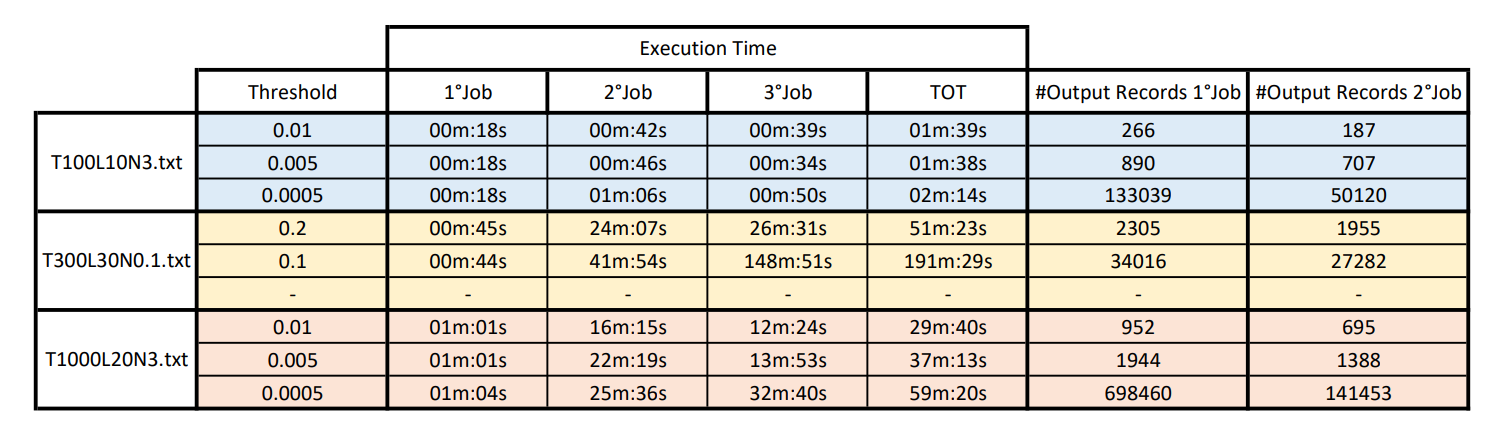
\includegraphics[scale=0.59]{./img/-t}}
   	\end{figure}
    \vspace{-0.5cm}
    \\
   	Considering a single dataset, it's clear that smaller is the support grater will be the execution time. If we compare different datasets results, it's possible to see that the performances don't depend entirely on the dataset size but mainly on the dataset structure (mean transaction length, number of different items,...). With longer transactions and an high number of occurrences wrt each singleton, we will have a greater computational load both in the second and last jobs. In particular, in the last job, the algorithm has to compare the list of common occurrences between the transactions-id list of all the items in a candidate itemset. This computation has to be done for all the candidates itemsets. Considering what just said, we can understand why the performances of the algorithm are, in general, more linked to the mean number of occurrences of a single item in the dataset then to the size of the datasets itself.  Despite the fact that \textit{T1000L20N3.txt} is about three time bigger then  \textit{T300L30N0.1.txt}, and despite the fact that, considering 0.0005 as support, it is also related to a number of candidates which is of one order of magnitude greater than the one of \textit{T300L30N0.1.txt} (for support 0.1), this last dataset candidates are likely to appear in a number of transactions which is about 2-3 order of magnitude greater than the ones of the candidates of \textit{T1000L20N3.txt}. These considerations are enough to explain the results seen in the image but, to be fair, we should have considered even the mean number of items in each candidate: from this point of view, looking at the results, the two datasets were pretty balanced. \\
   	The second parameter to be analyze has been the chunk size (\textbf{-c}). For these tests, the other parameters has been set to the default values except for the threshold which has been set to 0.0005 for both  \textit{T1000L20N3.txt} and  \textit{T100L10N3.txt} and to 0.1 for  \textit{T300L30N0.1.txt}. 
	\begin{figure}[h]
		\centering
		\subfloat[]{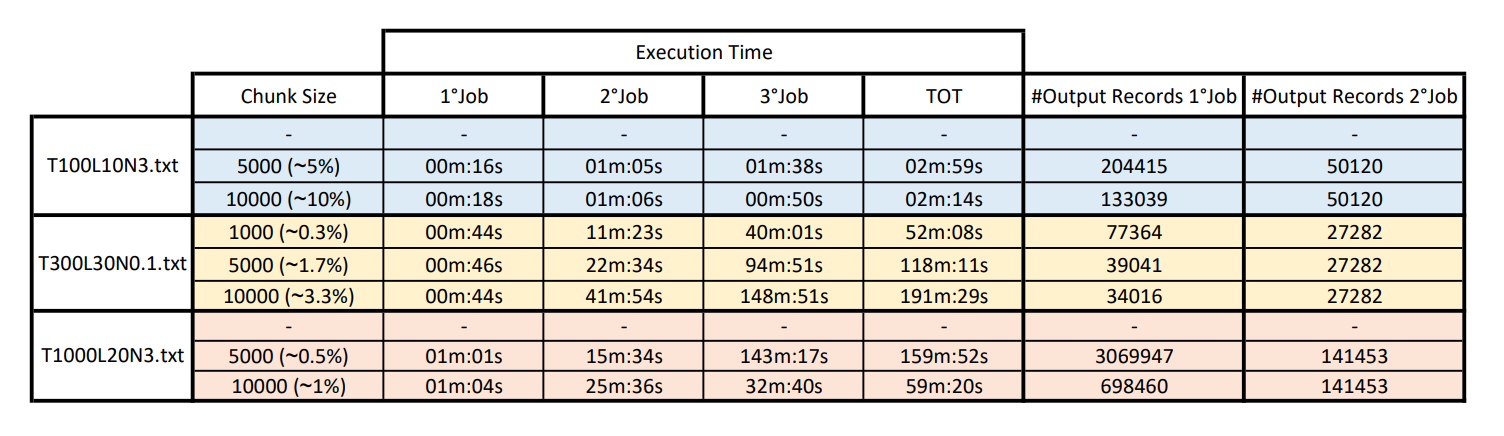
\includegraphics[scale=0.59]{./img/-c}}
	\end{figure}
	\vspace{-0.5cm}
	\\    	          	
   	The results shows how this parameter influences in different ways the execution time for the second and the last jobs. In fact, with a lower chunk size, the first job computational load could be drastically reduced. At the same time, in this scenario, we will have a lower (\textbf{scaled}) threshold value which determines an higher number of candidates to check in the last job thus an higher execution time should be expected for it. Depending on the dataset structure, we may want to choose the best value for this parameter in order to have a balanced computational load: to do this is necessary to have a prior knowledge about the input dataset. This parameter has been kept despite of this big constraint because, in general, is handy to have it even if the dataset structure is unknown.\\
   	What follows are the results related to the analysis of the parameters which determine the number of reducers for the different jobs.
   	The following table contains the results obtained by changing the number of reducers for the second job (=first extraction job).	  
   	\begin{figure}[h]
   		\centering
   		\subfloat[]{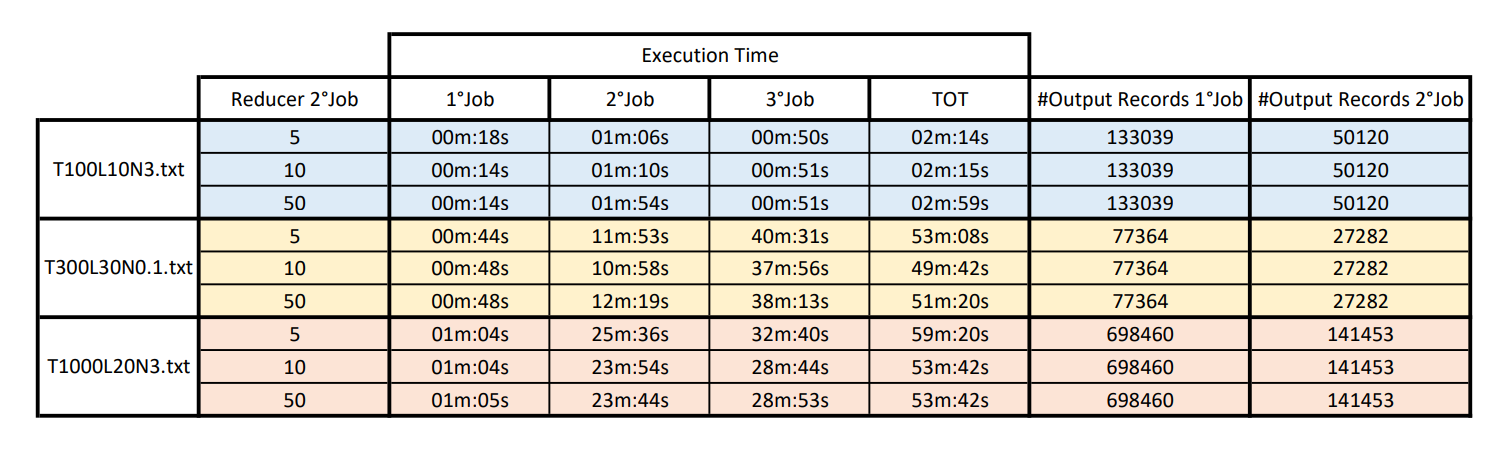
\includegraphics[scale=0.59]{./img/-r1}}
   	\end{figure}
   	\vspace{-0.55cm}
   	\\  	          	
   	This table shows, instead, the results obtained by changing the reducers number of the last job.
   	\begin{figure}[h]
   		\centering
   		\subfloat[]{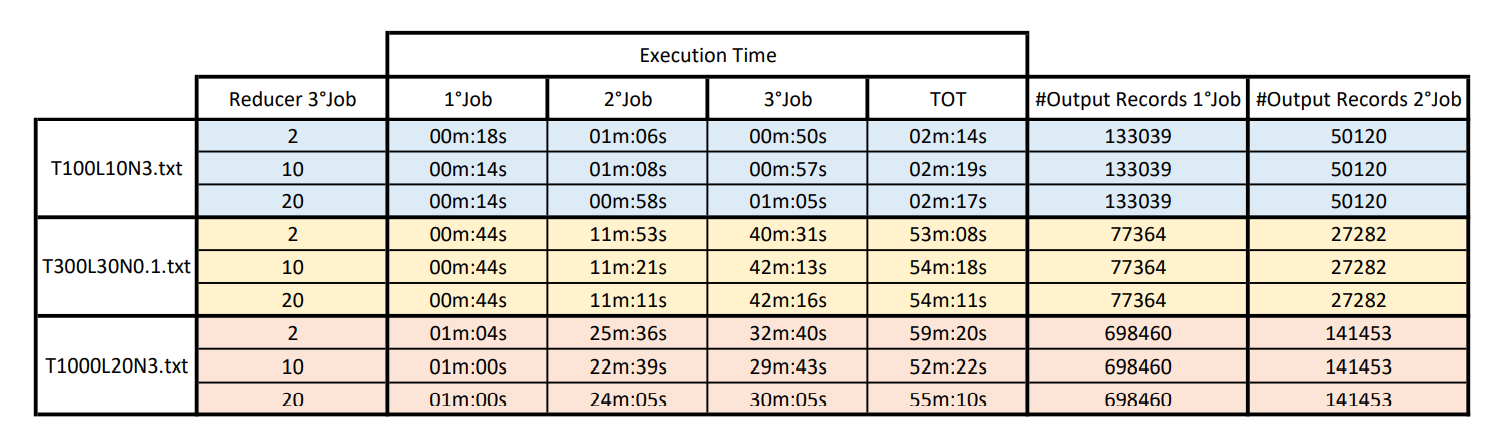
\includegraphics[scale=0.59]{./img/-r2}}
   	\end{figure}	
    \\
   	For these tests, the threshold parameters has been set to the same values as the previous test. For each datasets has been chosen, as chunk size, the best parameter found, again, in the previous test. The results show that both parameters have not an influence, wrt the execution time,
	in the tested scenarios. This has been an expected result considering that, according to the theoretical description and the actual implementation of the algorithm, both reducers have a marginal role in the whole computation. An other factor that partially contributes to reduce the influence of these two parameters is the fact that reduce tasks are almost ready to go as soon as the last map task end. This is because the framework starts to load data for the reduce tasks before the termination of all the map tasks thus, the overhead caused by the data loading for a configuration with less parallel reduce tasks, has a lower impact on the execution time. Surely, for huge datasets with a lot of candidates and/or many splits results to merge (with the last reducer), it's worth considering a higher number of reducers.      	
   	
   	\section*{Second Phase}
   	
   	This second phase has seen the comparison between the performances of SON algorithm described in this report and spmf Apriori. The datasets chosen for this comperison have been \textit{T1000L20N3.txt} and \textit{T100L10N3.txt}. To test spmf Apriori the following command has been used:
   	\begin{itemize}
   		\item \textbf{ java jar $<$jar-path$>$/spmf.jar run Apriori $<$input-file$>$ $<$outupt-file$>$ $<$val\%$>$}
   	\end{itemize}
   	Where:
   	\begin{itemize}	
   		\item \textbf{$<$..$>$:} represents a mandatory parameter.
   		\item \textbf{val\%:} represents the support threshold expressed as percentage.
   	\end{itemize}
   	The results obtained are shown in the following table.
   	\begin{figure}[h]
   		\centering
   		\subfloat[]{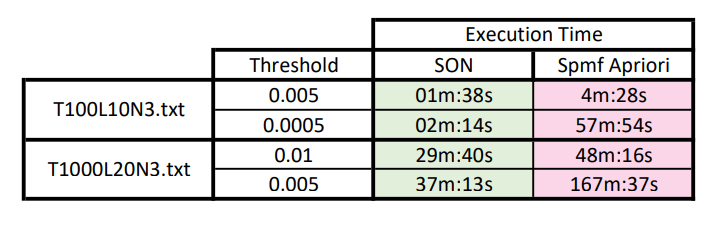
\includegraphics[scale=0.6]{./img/son-ap}}
   	\end{figure}
   	\vspace{-0.5cm}
   	\\ 
   	A low number of test cases has been checked (because of the high execution time of Apriori) but, from these few scenarios, a quite convincing trend can still be detected. The MR implementation of SON algorithm is, in general, a much better choice if we want to solve the "frequent itemset extraction" problem in less time. Supposing, for the sake of the argument, that the final frequent itemsets list is very small then the Apriori algorithm could perform better (depending on the size of the input dataset). But, considering that is not possible to know exactly how many frequent itemsets will be detected for a given dataset and a given threshold, SON algorithm still remains the preferable choice.     
   	
\end{document}          